\documentclass[enabledeprecatedfontcommands,fontsize=11pt,paper=a4,twoside]{scrartcl}

\newcommand*{\red}{\textcolor{red}}
\newcommand*{\blue}{\textcolor{blue}}
\newcommand*{\bbe}{\textcolor{bbe}}

\newcommand{\grad}{\ensuremath{^{\circ}} }
\renewcommand{\strut}{\vrule width 0pt height5mm depth2mm}

\setlength{\parindent}{0pt}

\usepackage[utf8]{inputenc}
\usepackage[T1]{fontenc}
\usepackage[final]{pdfpages}
% obere Seitenränder gestalten können
\usepackage{fancyhdr}
\usepackage{moreverb}
% Graphiken als jpg, png etc. einbinden können
\usepackage{graphicx}
\usepackage{stmaryrd}
% Floats Objekte mit [H] festsetzen
\usepackage{float}
% setzt URL's schön mit \url{http://bla.laber.com/~mypage}
\usepackage{url}
% Externe PDF's einbinden können
\usepackage{pdflscape}
% Verweise innerhalb des Dokuments schick mit " ... auf Seite ... "
% automatisch versehen. Dazu \vref{labelname} benutzen
\usepackage[ngerman]{varioref}
\usepackage[ngerman]{babel}
\usepackage{ngerman}
% Bibliographie
\usepackage{bibgerm}
\usepackage{svg}
% Tabellen
\usepackage{tabularx}
\usepackage{supertabular}
\usepackage[colorlinks=true, pdfstartview=FitV, linkcolor=blue,
            citecolor=blue, urlcolor=blue, hyperfigures=true,
            pdftex=true]{hyperref}
\usepackage{bookmark}



\newcounter{one}
\newcounter{two}[one]
\newcounter{three}[two]

\newcommand{\tone}{0\theone}
\newcommand{\ttwo}{0\thetwo}
\newcommand{\tthree}{0\thetree}
\newcommand{\one}{\stepcounter{one}0\theone}
\newcommand{\two}{\stepcounter{two}0\thetwo}
\newcommand{\three}{\stepcounter{three}0\thethree}
\newcommand\s{\rule{0pt}{4ex}}        
\newcommand{\cb}[1]{{\textcolor{blue}{#1}}}
\newcommand*{\hint}{\paragraph{\textcolor{blue}{Hinweise}}}
\newcommand*{\condition}{\paragraph{Voraussetzung}$\;$ \vspace{0.2cm}\\}
\newcommand*{\actions}{\paragraph{Vorgehen} $\;$\vspace{0.2cm}\\}
\newcommand*{\action}{\paragraph{Vorgehen}}
\newcommand*{\hdot}{\\ \hdashline[1pt/5pt]}
\newcommand*{\hdo}{.............}
\newcommand*{\aOne}{\textcolor{bbe}{Alternative 1:}}
\newcommand*{\aTwo}{\textcolor{bbe}{Alternative 2:}}
\newcommand*{\aThree}{\textcolor{bbe}{Alternative 3:}}
\newcommand*{\aFour}{\textcolor{bbe}{Alternative 4:}}



\usepackage{geometry}
\usepackage{hyperref}
\usepackage{pdfpages} 
\usepackage{colortbl}
%\usepackage{graphicx}   
%\usepackage[utf8x]{inputenc}
\usepackage{fmtcount}
\usepackage[ngerman]{babel}
\usepackage{booktabs}
\usepackage{fancyhdr}
\usepackage[T1]{fontenc}
\usepackage{nameref}
\usepackage{graphicx}
\usepackage{subfigure}


\pagestyle{fancy}
\fancyhf{}

%

%

%

%

\definecolor{dartmouthgreen}{rgb}{0.05, 0.5, 0.06}
\definecolor{color}{rgb}{0.67, 0.88, 0.69}
\definecolor{todo}{rgb}{1.0, 0.41, 0.71}
\definecolor{sort}{rgb}{0.45, 0.76, 0.98}
\definecolor{prob}{rgb}{0.74, 0.83, 0.9}
\definecolor{anw}{rgb}{0.94, 0.86, 0.51}
\definecolor{ghostwhite}{rgb}{0.97, 0.97, 1.0}
\definecolor{glaucous}{rgb}{0.38, 0.51, 0.71}
\definecolor{bbe}{rgb}{0.13, 0.67, 0.8}
\usepackage{amsmath}
\usepackage{tabularx}
\usepackage{setspace} 
\hypersetup{
	colorlinks = true,
	linkbordercolor = {white},
	linkcolor=dartmouthgreen,          % color of internal links (change box color with linkbordercolor)
	citecolor=red,        % color of links to bibliography
	filecolor=magenta,      % color of file links
	urlcolor=cyan 
}
\usepackage{geometry}
\geometry{
	a4paper,
	left=20mm,
	right=20mm,
	top=2cm,
	bottom=4cm,
	footskip=4cm
}


\addtolength{\headwidth}{20mm}
\addtolength{\headheight}{2\baselineskip}
\addtolength{\headheight}{0.61pt}


\renewcommand{\headrulewidth}{0pt}
\renewcommand{\headrule}{\vbox to 0pt{\rule{\headwidth}{0.2pt}}}
\setlength{\headsep}{30pt}


\let\tempone\itemize
\let\temptwo\enditemize
\renewenvironment{itemize}{\tempone\addtolength{\itemsep}{-10.0pt}}{\temptwo}

\let\origenumerate\enumerate
\let\origendenumerate\endenumerate
\renewenvironment{enumerate}{\origenumerate \addtolength{\itemsep}{-10.0pt}}{\origendenumerate}

%\addtolength{\itemsep}{-10.0pt}
%\setitemize{itemsep=-10.0pt}
%\setenumerate{itemsep=-10.0pt}

\hyphenation{Arbeits-paket}

% Damit Latex nicht zu lange Zeilen produziert:
%\sloppy
%Uneinheitlicher unterer Seitenrand:
%\raggedbottom

% Kein Erstzeileneinzug beim Absatzanfang
% Sieht aber nur gut aus, wenn man zwischen Absätzen viel Platz einbaut
%\setlength{\parindent}{0ex}

% Abstand zwischen zwei Absätzen
%\setlength{\parskip}{1ex}

% Seitenränder für Korrekturen verändern
%\addtolength{\evensidemargin}{-1cm}
%\addtolength{\oddsidemargin}{1cm}

%\bibliographystyle{gerapali}

% Lustige Header auf den Seiten
  \pagestyle{fancy}
  \setlength{\headheight}{70.55003pt}
  \fancyhead{}
  \fancyhead[LO,RE]{Software--Projekt 2\\ WiSe 2018/2019
  \\Architekturbeschreibung}
  \fancyhead[LE,RO]{Seite \thepage\\\slshape \leftmark\\\slshape \rightmark}

%
% Und jetzt geht das Dokument los....
%

\begin{document}

% Lustige Header nur auf dieser Seite
  \thispagestyle{fancy}
  \fancyhead[LO,RE]{ }
  \fancyhead[LE,RO]{Universität Bremen\\FB 3 -- Informatik\\
  Prof. Dr. Rainer Koschke \\TutorIn: Marcel Steinbeck}
  \fancyfoot[C]{}

% Start Titelseite
  \vspace{3cm}

  \begin{minipage}[H]{\textwidth}
  \begin{center}
  \bf
  \Large
  Software--Projekt 2 WiSe 2018/2019\\
  \smallskip
  \small
  VAK 03-BA-901.02\\
  \vspace{3cm}
  \end{center}
  \end{minipage}
  \begin{minipage}[H]{\textwidth}
  \begin{center}
  \vspace{1cm}
  \bf
  \Large Benutzerhandbuch - GraphIt \\
  TeamBlank \\
  \vspace{2cm}
  
\includegraphics[width=3.0in]{logo_graphit.png}

  
  \end{center}
 
  \end{minipage}
  \vfill
  \begin{minipage}[H]{\textwidth}
  \begin{center}
  \sf
  \begin{tabular}{lr}
  Anthony Mendil & antmen@tzi.de \\
  Bastian Rexhäuser & brexhaeu@tzi.de\\
  Clement Phung & clement1@tzi.de \\
  Jacky Philipp Mach & machja@tzi.de \\
  Jonah Jaeger & jjaeger@tzi.de \\
  Nina Unterberg & nin\_unt@tzi.de \\
  \end{tabular}
  \\ ~
  \vspace{2cm}
  \\
  \it Abgabe: 10. März 2019 --- Version 1.0\\ ~
  \end{center}
  \end{minipage}

% Ende Titelseite

% Start Leerseite

\newpage

  \thispagestyle{fancy}
  \fancyhead{}
  \fancyhead[LO,RE]{Software--Projekt \\  2018/2019
  \\Benutzerhandbuch}
  
  \fancyhead[LE,RO]{Seite \thepage\\\slshape \leftmark\\~}
  \fancyfoot{}
  \renewcommand{\headrulewidth}{0.4pt}
  \tableofcontents

\newpage

  \fancyhead[LE,RO]{Seite \thepage\\\slshape \leftmark\\\slshape \rightmark}

%%%%%%%%%%%%%%%%%%%%%%%%%%%%%%%%%%%%%%%%%%%%%%%%%%%%%%%%%%%%%%%%%%%%%%%%
%%%%%%%%%%%%%%%%%%%%%%%%%%%%%%%%%%%%%%%%%%%%%%%%%%%%%%%%%%%%%%%%%%%%%%
\section*{Vorwort}
Mit diesem Handbuch wird die Bedienung der Software \textbf{GraphIt} beschrieben. Diese Anwendung wurde im Rahmen des Moduls \glqq{Softwareprojekt 2}\grqq im Wintersemester 2018/19 entwickelt und ist zur Erstellung, Editierung und Visualisierung von Wirkungsdiagrammen für den Syndromansatz entworfen worden. \\
Eine Nutzung des Programms für Zwecke, die von dem angedachten Einsatzbereich abweicht ist möglich. Allerdings wird in diesem Dokument nicht weiter auf eine solche Nutzung eingegangen. Bei dieser Nutzung, die nicht dem angedachten Einsatz entspricht, ist ferner zu berücksichtigen, dass eventuell gewisse Funktionen wünschenswert wären, die aufgrund der Anforderungen jedoch bewusst nicht eingebaut wurden. Insbesondere sind hier die Regeln zu beachten, die für die Erstellung von Wirkungszusammenhängen gemäß des Syndromansatzes gelten. \\
Bei der vorliegenden Software handelt es sich um eine Neu-Entwicklung. Somit existieren keinerlei Vorversionen, mit denen der Funktionsumfang oder die Bedienung der Software in diesem Dokument verglichen werden könnte. 

%%%%%%%%%%%%%%%%%%%%%%%%%%%%%%%%%%%%%%%%%%%%%%%%%%%%%%%%%%%%%%%%%%%%%%%%
%%%%%%%%%%%%%%%%%%%%%%%%%%%%%%%%%%%%%%%%%%%%%%%%%%%%%%%%%%%%%%%%%%%%%%
\section{Einführung}
\subsection{Adressierte Leser}
Dieses Handbuch richtet sich an alle Nutzer, die \textbf{GraphIt} für ihren bestimmungsgemäßen Einsatz verwenden möchten. Dieser umfasst die Erstellung, Bearbeitung und Auswertung von Wirkungszusammenhängen gemäß des Syndromansatzes. Die Software ist sowohl für Anfänger geeignet, die noch nie oder nur sehr selten mit einem vergleichbaren Programm gearbeitet haben, als auch für Fortgeschrittene und Experten, die über mehr Erfahrung in der Bedienung ähnlicher Software verfügen. \\
Von dem Adressatenkreis des vorliegenden Dokuments wird die Kenntnis der Terminologie des Syndromansatzes erwartet.  
\subsection{Verwandte Dokumente}
Neben dem Benutzerhandbuch der Software \textbf{GraphIt}, existiert ebenfalls ein Testprotokoll, welches die Entwickler erstellt haben, um die Korrektheit der Software zu garantieren. Außerdem eine Architekturbeschreibung die detaillierteren Einblick in die Architektur der Software gewährt. 
\subsection{Konventionen}
\begin{itemize}
	\item Wenn im Verlaufe des Dokumentes von einem Graphen die Rede ist, wird sich auf ein Wirkungsdiagramm  gemäß des Syndromansatzes bezogen.
\end{itemize}

\subsection{Informationen über die Verwendung des Dokuments}

\begin{itemize}
	\item Alle eingebundenen Screenshots in das Dokument wurden auf einem Computer mit Windows 10 Betriebssystem aufgenommen. Wenn ihre Darstellung der Software leicht von den gerade erwähnten Screenshots abweicht, bitten wir dies zu entschuldigen.
	\item Um die Software \textbf{GraphIt} am Besten verstehen und anwenden zu können, empfehlen wir das Dokument von Anfang bis Ende durchzuarbeiten, da sich manche Einträge auf vorherige beziehen. 
\end{itemize}



%%%%%%%%%%%%%%%%%%%%%%%%%%%%%%%%%%%%%%%%%%%%%%%%%%%%%%%%%%%%%%%%%%%%%%
\newpage
\section{Installation und Starten des Programms} \label{sec:installation}

\subsection{Installationsvoraussetzungen}
\subsubsection{Java 8}
\red{TODO}

\subsection{Installationsanweisungen}
\begin{itemize}
	\item \red{TODO}
\end{itemize}
\subsection{Starten des Programms}
\red{TODO}

\newpage	
%%%%%%%%%%%%%%%%%%%%%%%%%%%%%%%%%%%%%%%%%%%%%%%%%%%%%%%%%%%%%%%%%%%%%		
\section{Benutzeroberfläche}
\subsection{Tasten-/ Mausbelegungen}

\begin{tabular} {|p{8cm}|p{8cm}|}
	\hline
	\rowcolor{glaucous}\multicolumn{2}{|l|} {\parbox{16cm}{\textbf{\textcolor{ghostwhite}{Maus-/ Tastenbelegungen}}} } \\ \hline\hline 	
	Drucken	& Ctrl + P \\ \hline
	Neue Datei	& Ctrl + N \\ \hline
	GXL importieren	& Ctrl + Shift + I \\ \hline
	Speichern unter	&	Ctrl + S \\ \hline
	\red{TODO} & \\ \hline
\end{tabular}

 
\subsection{Übersicht}
1\hdo..Auswählen \\
2\hdo..Sphäre hinzufügen \\
3\hdo..Sphäre löschen \\
4\hdo..Sphäre vergrößern \\
5\hdo..Sphäre verkleinern \\
6\hdo..Hintergrundfarbe der Sphäre verändern  \\
7\hdo..Schriftart der Sphäre verändern  \\
8\hdo..Schriftgröße der Sphäre verändern \\
9\hdo..Automatische Anordnung \\
10\hdo  Symptom hinzufügen \\
11\hdo  Symptom löschen \\
12\hdo  Symptom vergrößern \\
13\hdo  Symptom verkleinern \\
14\hdo  Hintergrundfarbe des Symptoms verändern \\
15\hdo  Randfarbe des Symptoms verändern \\
16\hdo  Form des Symptoms verändern \\
17\hdo  Automatische Anordnung \\
18\hdo  Schriftart des Symptoms verändern \\
19\hdo  Schriftgröße des Symptoms verändern \\
20\hdo  Ankerpunkte ein-/ ausblenden \\
21\hdo  Relation löschen \\
22\hdo  Ankerpunkt löschen \\
23\hdo  Farbe der Relation verändern \\
24\hdo  Art der Relation  verändern \\
25\hdo  Pfeilspitze der Relation verändern \\
26\hdo Bearbeiter-Modus\\
27\hdo Ersteller-Modus\\
28\hdo Analyse-Modus\\
29\hdo Rückgängig \\
30\hdo Wiederherstellen\\
31\hdo Hervorgehobene Elemente aktivieren\\
32\hdo Element hervorheben\\
33\hdo Hervorhebung von Element entfernen\\
34\hdo Ausgeblendete Elemente aktivieren\\
35\hdo Elemente ausblenden\\
36\hdo Ausblendung von Element entfernen\\
37\hdo  Vorlage- Regeln\\
38\hdo  Maximale Sphären\\
39\hdo  Maximale Symptome\\
40\hdo  Maximale Relationen\\
41\hdo  Relationstyp erlauben\\
42\hdo  Sperrende Elemente: Sphäre\\
43\hdo  Sperrende Elemente: Symptom\\
44\hdo  Sperrende Elemente: Relation\\
45\hdo Aktuelle Mausposition \\
46.1..........Nach der Pfeilspitze der Relation filtern \\
46.2..........Nach regulären Ausdruck filtern\\
47.1..........Zoom Fenster  \\
47.2..........Zoom-leiste \\
48\hdo  Übersicht \\
49\hdo Neue Datei hinzufügen\\
50\hdo Datei öffnen\\
51\hdo Speichern unter\\
52\hdo Drucken\\
53\hdo GraphIt schließen\\
54\hdo Als Vorlage exportieren\\
55\hdo Als GXL exportieren\\
56\hdo Als PDF exportieren\\
57\hdo Als Verlaufsprotokoll exportieren\\
58\hdo Als Vorlage importieren\\
59\hdo Als GXL importieren\\
60\hdo Sprache\\
61\hdo Sprache Benutzeroberfläche\\
62\hdo Sprache des Graphen\\
63\hdo Dokumentation\\
64\hdo über uns \\
65\hdo Graphmaße\\
66\hdo Vorgänger/ Nachfolger\\
67\hdo Anzahl\\
68\hdo Kürzester Weg/ alle Wege\\
69\hdo Analyse-Optionen: Pfeilketten, Konvergente/ Divergente Verzweigungen, Verzweigungen,\\ 		
\hspace*{1.7cm} Zyklen\\
70\hdo Verlauf\\
71\hdo Den Verlauf neu laden\\
72\hdo Den Verlauf nach einer Aktion filtern\\ 


\begin{landscape}
	\begin{figure}
		\centering
		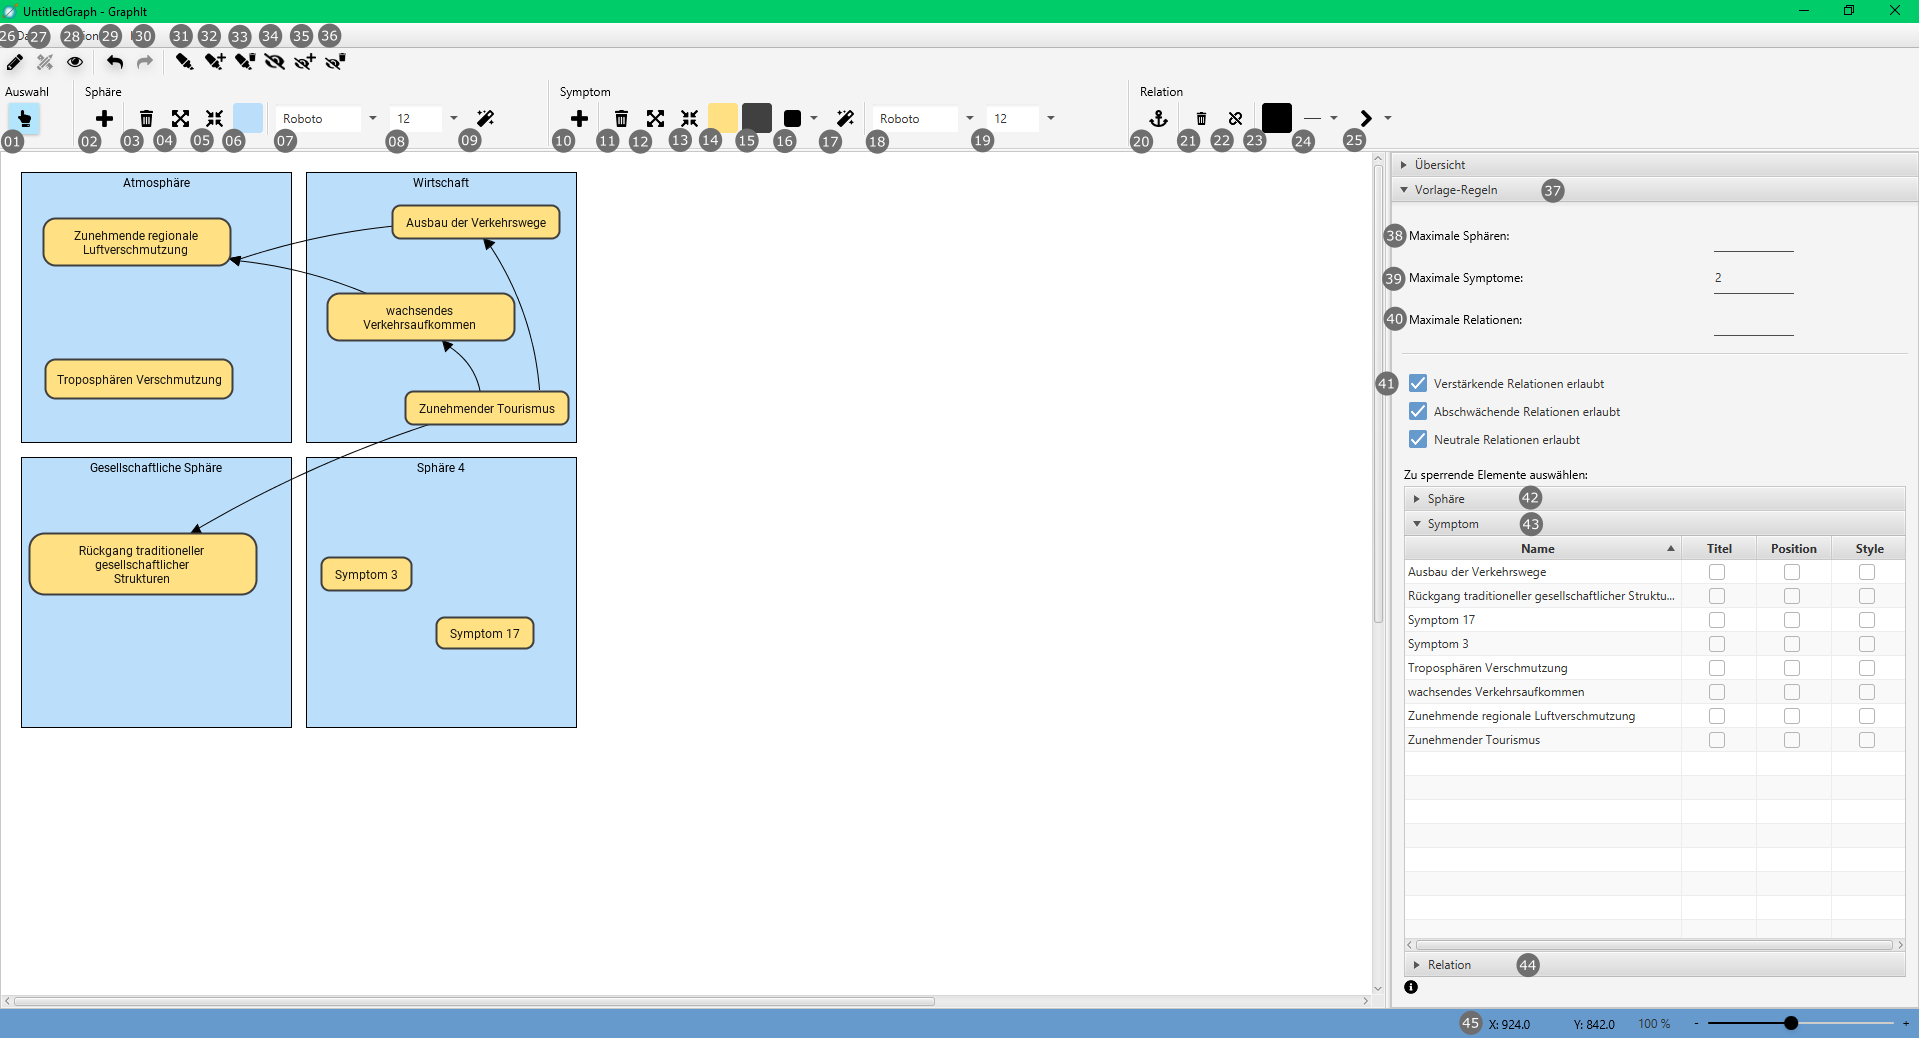
\includegraphics[width=22cm]{over.png}
		\caption{Übersicht über den Ersteller Modus}
	\end{figure}
\end{landscape}
\begin{landscape}
	\begin{figure}
		\centering
		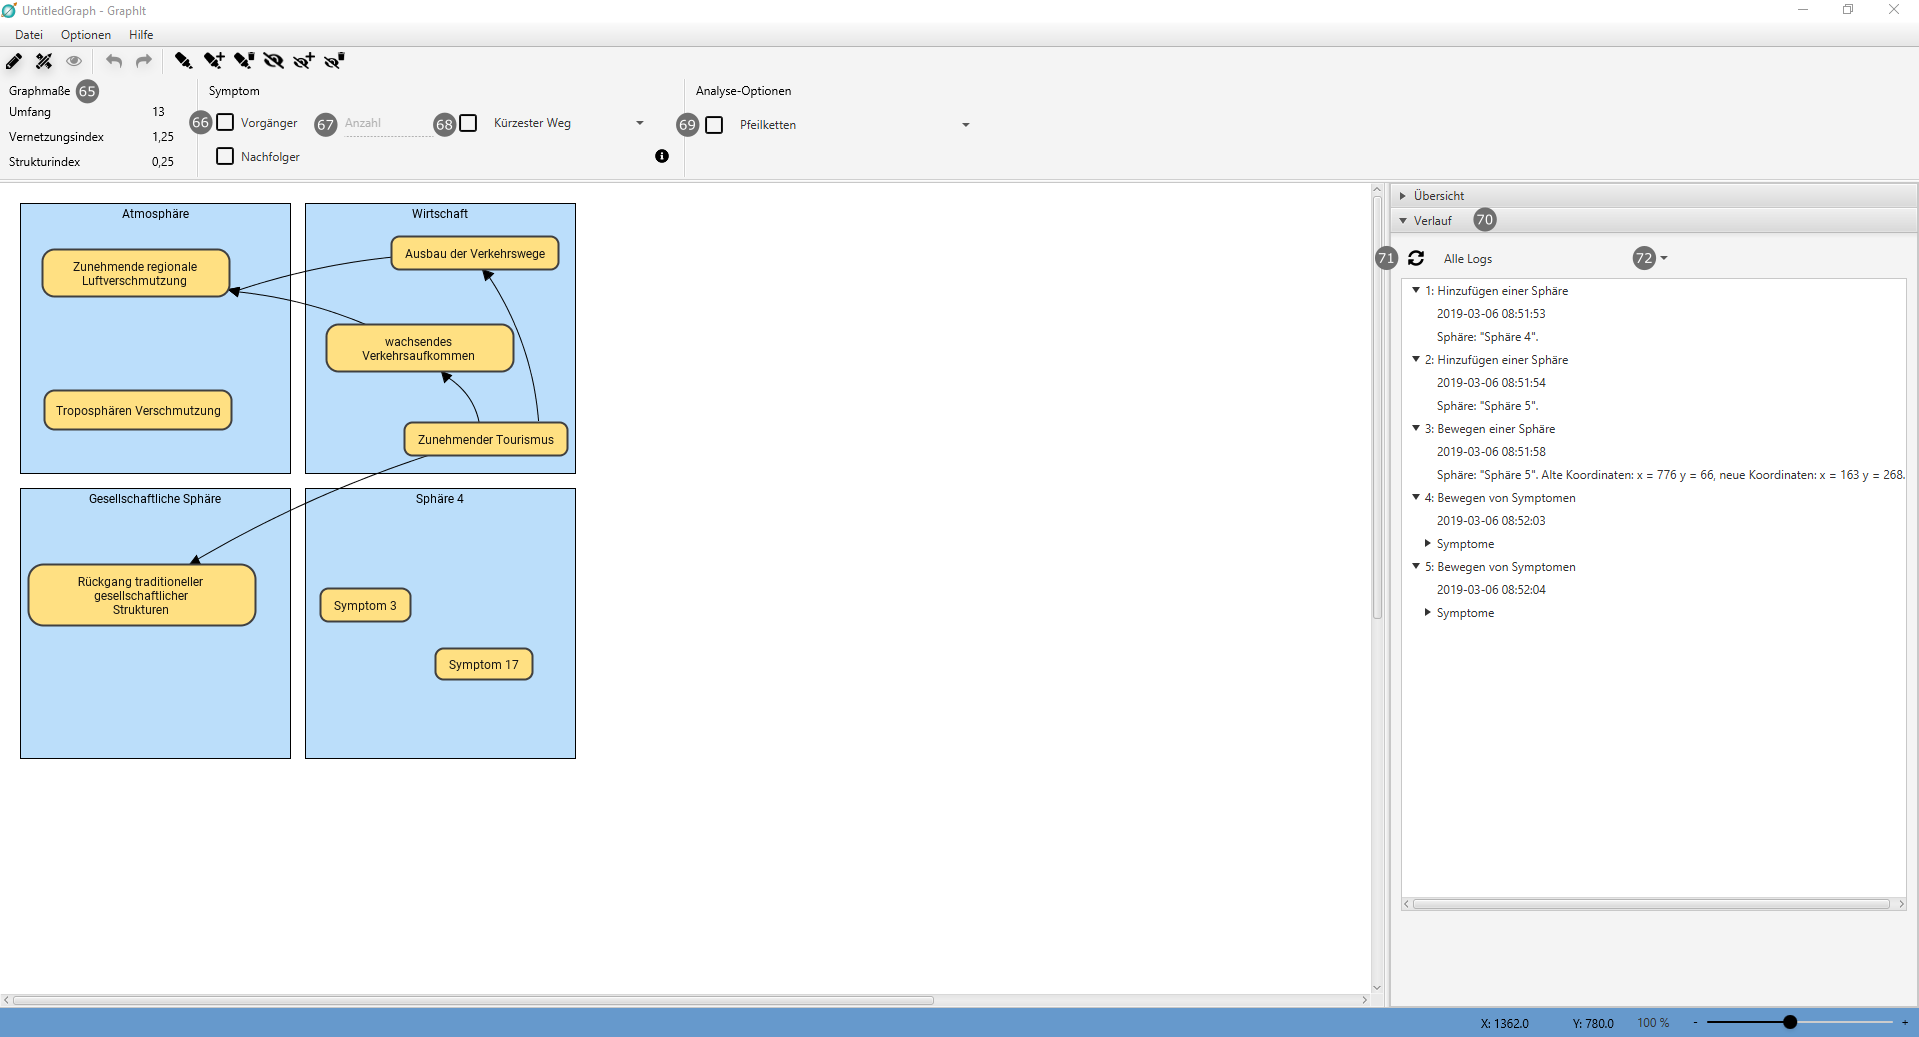
\includegraphics[width=22cm]{over2.png}
		\caption{Übersicht über den Analyse Modus}
	\end{figure}
\end{landscape}

\begin{figure}[ht!]
	\centering
	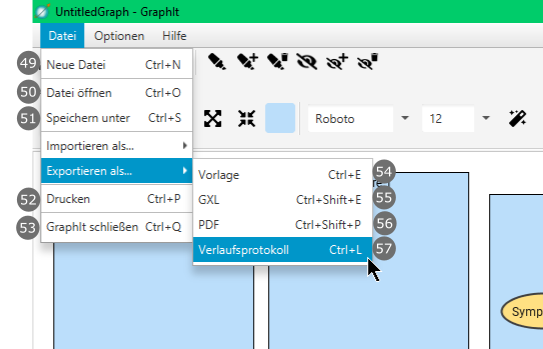
\includegraphics[width=0.5\columnwidth, keepaspectratio]{menu1.png} 
	\caption{Menü (1)}
\end{figure}

\begin{figure}[ht!]
	\centering
	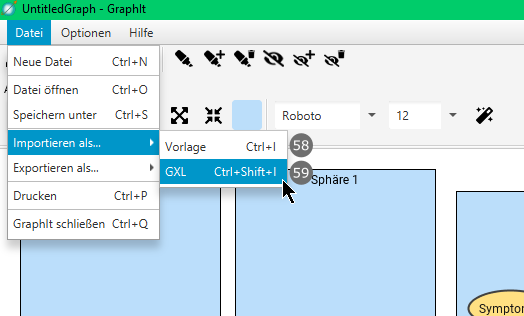
\includegraphics[width=0.5\columnwidth, keepaspectratio]{menu4.png} 
	\caption{Menü (2)}
\end{figure}

\begin{figure}[ht!]
	\centering
	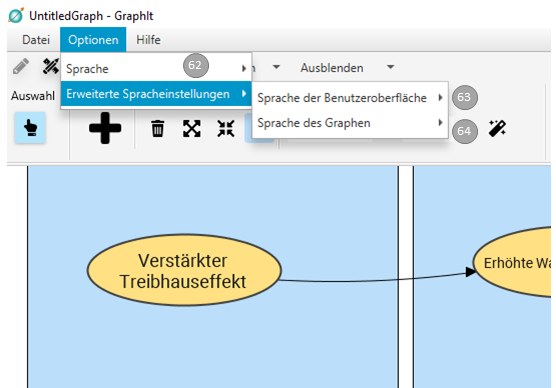
\includegraphics[width=0.5\columnwidth, keepaspectratio]{menu2.png} 
	\caption{Menü (3)}
\end{figure}

\begin{figure}[ht!]
	\centering
	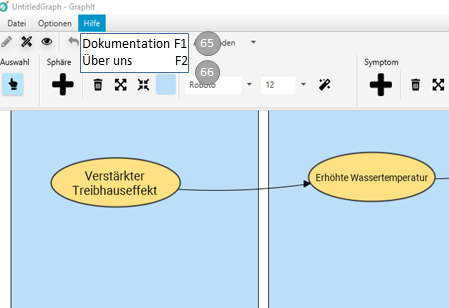
\includegraphics[width=0.5\columnwidth, keepaspectratio]{menu3.png} 
	\caption{Menü (4)}
\end{figure}


\begin{figure}[ht!]
	\centering
	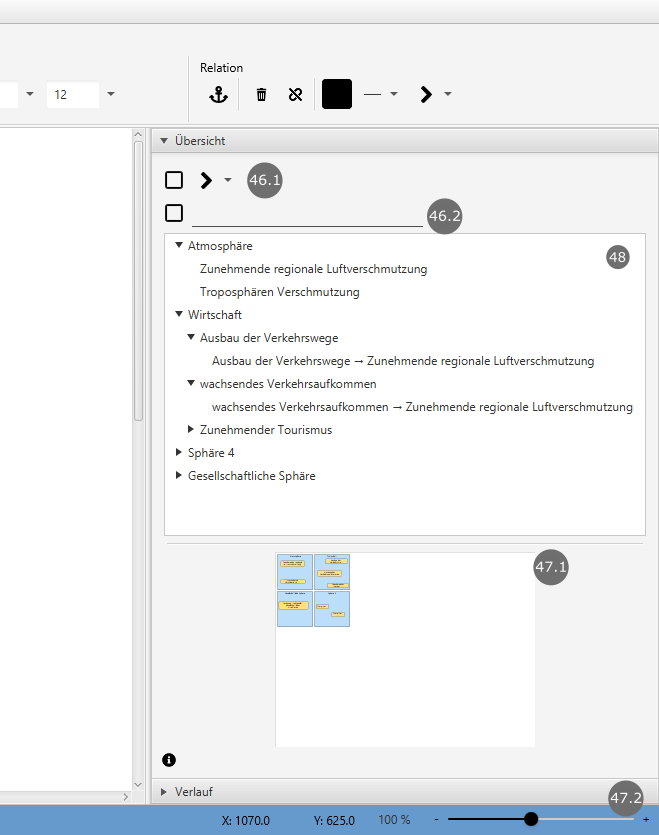
\includegraphics[width=0.5\columnwidth, keepaspectratio]{side.png} 
	\caption{Übersicht}
\end{figure}







\clearpage	
%%%%%%%%%%%%%%%%%%%%%%%%%%%%%%%%%%%%%%%%%%%%%%%%%%%%%%%%%%%%%%%%%%%%%%	
\section{Übersicht} \label{sec:uebersicht}
\subsection{Ersteller Modus}
Im \texttt{Ersteller Modus} kann der Benutzer einen Syndromansatz erstellen und editieren. Im Unterschied zu dem \nameref{sec:editor} kann der Benutzer Vorlageregel für den aktuellen Syndromansatz hinterlegen. Diese werden erst auf dem Graphen im \nameref{sec:editor} angewandt. 


\subsubsection{Relevante Kapitel}
\begin{itemize}
	\item \nameref{pick}
	\item \nameref{edit}
	\item \nameref{sphere}	
	\item \nameref{symptom}	
	\item \nameref{relations}	
	\item \nameref{template}
	\item \nameref{overwiew}
	\item \nameref{zoom}
	\item \nameref{export}
	\item \nameref{import}
	\item \nameref{print}
	\item \nameref{dialog}
	\item \nameref{fehlermeldungen}
	\item \nameref{settings}	
\end{itemize}
\subsection{Bearbeiter Modus} \label{sec:editor}
Im \texttt{Bearbeiter Modus} kann der Benutzer einen Syndromansatz erstellen und bearbeiten. Die Bearbeitung des Graphen folgt den hinterlegten Vorlageregeln. Alle Aktionen auf dem Graph werden geloggt, d.h. ein Verlaufsprotokoll erstellt, welches ebenfalls einsehbar und exportierbar/ importierbar ist. 
\subsubsection{Relevante Kapitel}
\begin{itemize}
	\item \nameref{pick}
	\item \nameref{edit}
	\item \nameref{sphere}	
	\item \nameref{symptom}	
	\item \nameref{relations}	
	\item \nameref{logs}
	\item \nameref{overwiew}
	\item \nameref{zoom}
	\item \nameref{export}
	\item \nameref{import}
	\item \nameref{print}
	\item \nameref{dialog}
	\item \nameref{fehlermeldungen}
	\item \nameref{settings}	
\end{itemize}
\subsection{Analyse Modus}
Im \texttt{Analyse Modus} kann ein Syndromansatz analysiert und ausgewertet werden. In diesem Modus ist keine Bearbeitung des Graphen möglich. \\
Die Analyse umfasst z.B. die Lokalisierung von Pfeilketten oder die Berechnung des kürzesten Weges zwischen 2 Symptomen. \\
Die Auswertung der Nutzerinteraktionen ist ebenfalls möglich. Diese können vom Benutzer gefiltert und angezeigt werden. 
\subsubsection{Relevante Kapitel}
\begin{itemize}
	\item \nameref{pick}	
	\item \nameref{logs}
	\item \nameref{overwiew}
	\item \nameref{zoom}
	\item \nameref{export}
	\item \nameref{import}
	\item \nameref{print}
	\item \nameref{dialog}
	\item \nameref{fehlermeldungen}
	\item \nameref{settings}	
	\item \nameref{analyse}
\end{itemize}

%%%%%%%%%%%%%%%%%%%%%%%%%%%%%%%%%%%%%%%%%%%%%%%%%%%%%%%%%%%%%%%%%%%%%%%

\newpage
\section{Instruktionen zur Nutzung des Programms} \label{sec:nutzung}

		\subsection{Auswahl von Graphelementen} \label{pick}
	\subsubsection{Eines Elements}
	\condition
	Es muss ein Syndrom mit mindestens einem Element (eine Sphäre/ ein Symptom/ eine Relation), welches ausgewählt werden soll, existieren. 
	\actions
	\aOne 
	\begin{enumerate}
		\item In der Menüleiste den Button \textit{Auswahl} durch einen Links-Klick aktivieren. 
		\item Den Cursor auf das Element bewegen und die linke Maustaste klicken. 
	\end{enumerate}
	\aTwo
	\begin{enumerate}
		\item In der Übersichtleiste das auszuwählende Element durch einen Links-Klick auswählen. 
	\end{enumerate}
	\hint
	\begin{itemize}
		\item Eine Relation kann manchmal etwas schwierig auszuwählen sein, da die Kanten vergleichsweise relativ dünn sind. 
		\item Die Nutzung der eben angesprochenen Übersichtsleiste wird in einem folgenden Unterkapitel (\ref{overwiew}) noch genauer beschrieben.
		\item Ausgewählte Elemente werden in der Visualisierung durch einen dickere Umrandung hervorgehoben.
	\end{itemize}
	
	\begin{figure}[ht!]
		\centering
		\subfigure[Alternative 1]{
			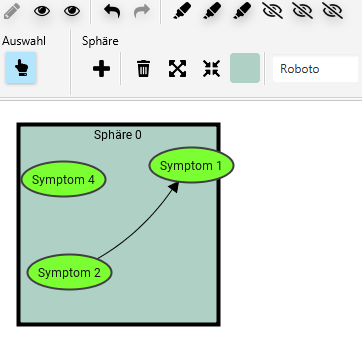
\includegraphics[width=0.4\columnwidth, keepaspectratio]{pick.png} 
		}
		\subfigure[Alternative 2]{
			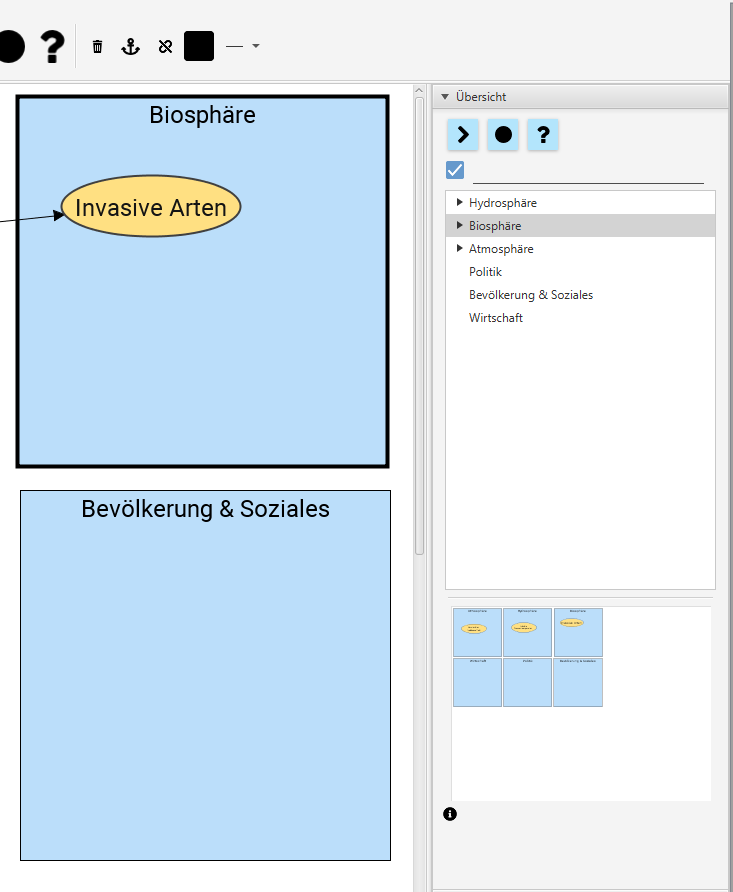
\includegraphics[width=0.4\columnwidth, keepaspectratio]{pick2.png} 
		}
		\caption{Auswahl}
		
	\end{figure}	

	
	%%%%%%%%%%%%%%%%%%%%%%%%%%%%%%%%%%%%%%%%%%%%%%%%%%%%%%%%%%%%%%%%%%%%%%% 	
	
	\newpage
	\subsubsection{Mehrerer Elemente}
	\condition
	Es muss ein Syndrom mit mindestens zwei Elemente (Sphären/ Symptome/ Relationen), welches ausgewählt werden soll, existieren. 
	\action
	\begin{enumerate}
		\item In der Menüleiste den Button \textit{Auswahl} durch einen Links-Klick aktivieren. 
		\item Auf der Tastatur den die Taste \texttt{Shift} gedrückt halten. 
		\item Den Cursor auf das Element bewegen, welches zur Auswahl hinzugefügt werden soll, und die linke Maustaste klicken. 
		\item Die \texttt{Shift} Taste solange gedrückt halten, wie Elemente der Auswahl hinzugefügt werden sollen.
		\item Die \texttt{Shift} Taste loslassen.
	\end{enumerate}
	\hint
	\begin{itemize}
		\item Verschiedene Arten (Sphären/ Symptome/ Relationen) von Graphelementen können in einer Aktion der Auswahl hinzugefügt werden. 
		\item Alle Aktionen bezüglich der Editierung des Graphen können auch auf mehrere Elemente gleichzeitig angewendet werden. \\
	\end{itemize}

	\subsubsection{Auswahl löschen}
	\red{TODO}
	
		\newpage
%%%%%%%%%%%%%%%%%%%%%%%%%%%%%%%%%%%%%%%%%%%%%%%%%%%%%%%%%%%%%%%%%%%%%%%%%%%%%%%%%%%%%%%%%%%%%%%%%%%%%%%%
		\subsection{Nutzung der Übersichtsleiste} \label{overwiew}
		Die Übersichtsleiste befindet sich am rechten Rand der Anwendung. Über diese Leiste kann ein Element des Syndroms sowohl ausgewählt als auch dessen Eigenschaften verändert werden. Des weiteren kann es als zusätzliche Hilfe herangezogen werden, um die Struktur des Syndroms zu untersuchen. \\
		So kann über diese Leiste (zusätzlich zur visuellen Darstellung des Syndroms) ermittelt werden, welche Sphäre, welche Symptome enthält und welche Symptome durch Relationen verbunden sind. In diesem Fenster ist auch ein Filter integriert. Die Filterfunktion kann durch entsprechende Eingaben die Beschriftung von Symptomen und die Relationstypen der Relationen filtern.
		
		\begin{figure}[ht!]
			\centering
			\subfigure{
				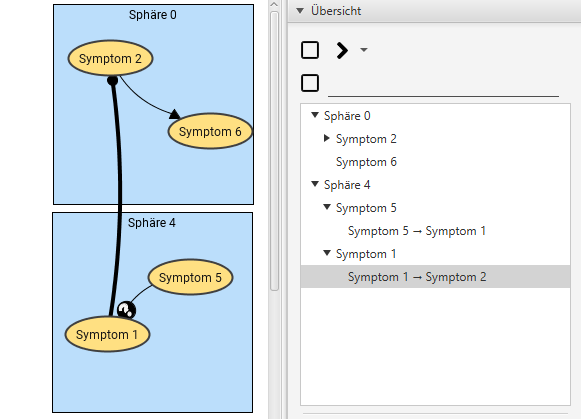
\includegraphics[width=0.4\columnwidth, keepaspectratio]{ubersicht.png} 
			}
			\caption{Übersichtsleiste}
			
		\end{figure}


%%%%%%%%%%%%%%%%%%%%%%%%%%%%%%%%%%%%%%%%%%%%%%%%%%%%%%%%%%%%%%%%%%%%%%%%%%%%%%%%%%%
\subsubsection{Navigation}		
	\condition
	Es muss ein Syndrom mit mindestens einer Sphäre im Programm geöffnet sein, damit die Übersichtsleiste nicht leer ist. 
	\action
	\begin{enumerate}
		\item In der Übersichtsleiste die Sphäre, zu der man die ihre zugeordneten Symptome angezeigt bekommen möchte, ausklappen. 
		\item Zum Schließen der Liste der Symptome die Sphäre einklappen. 
		\item Alternativ ein Symptom ausklappen, um die Liste der Relationen, die von ihm ausgehen, angezeigt zu bekommen. 
	\end{enumerate}
	\hint
	\begin{itemize}
		\item Element in der Übersichtsleiste können entweder durch einen Doppelklick der linken Maustaste oder durch einen Links-Klick auf das danebenstehende Pfeilsymbol ausgeklappt/ eingeklappt werden. 
		\item Ist in der Übersichtsleiste kein Pfeil vor einem Eintrag eingeblendet, so lässt sich dieses nicht ein-/ausklappen.
		\item Die Elemente eines Syndroms werden durch ihre Bezeichnung in der Übersichtleiste repräsentiert. Die Relationen werden durch ihr ausgehendes/ eingebendes Symptom identifiziert.\\
	\end{itemize}
		 
%%%%%%%%%%%%%%%%%%%%%%%%%%%%%%%%%%%%%%%%%%%%%%%%%%%%%%%%%%%%%%%%%%%%%%%%%%%%%%%%%%%
\subsubsection{Auswahl von Graphelementen}		
	\condition
	Es muss ein Syndrom mit mindestens einer Sphären im Programm geöffnet sein, damit die Übersichtsleiste nicht leer ist. 
	\action
	\begin{enumerate}
		\item In der Übersichtsleiste auf die eben beschriebene Weise bis zu der gewünschten Tiefe (nur Sphären, Symptome zu einer Sphäre, Relationen zu einem Symptom) navigieren. Dort das gewünschte Element wahlweise mit einem einfachen Links-Klick oder einem Doppelklick auswählen.
		\end{enumerate}
	\hint
	\begin{itemize}
		\item Das jeweils aktuell in der Übersichtsleiste ausgewählte Element wird auch in der (visuellen) Darstellung des Syndroms ausgewählt.\\
	\end{itemize}
		
%%%%%%%%%%%%%%%%%%%%%%%%%%%%%%%%%%%%%%%%%%%%%%%%%%%%%%%%%%%%%%%%%%%%%%%%%%%%%%%%%%%
\subsubsection{Filtern}
	\condition
	Es muss ein Syndrom mit mindestens einer Sphären im Programm geöffnet sein, damit die Übersichtsleiste nicht leer ist. 
	\actions
	\bbe{Filtern der Relationstypen:}
	\begin{enumerate}
		\item In der Übersichtsleiste einen Links-Klick in die Check-Box neben dem \textit{Nach der Pfeilspitze der Relation filtern}-Button ausführen, sodass dort ein Häkchen gesetzt ist.
		\item In der Übersichtsleiste einen Links-Klick auf den Button \textit{Nach der Pfeilspitze der Relation filtern} das Drop-Down-Menü dieses Buttons öffnen.
		\item In dem Drop-Down-Menü, den Relationstyp, der gefiltert werden soll, mit einem Links-Klick auswählen.
		\item Um wieder die Relationen aller Relationstypen einzublenden, erneut einen Links-Klick in die Check-Box neben dem \textit{Nach der Pfeilspitze der Relation filtern}-Button ausführen, sodass der Haken in dieser Box verschwindet.
	\end{enumerate}
	\bbe{Filtern der Symptome durch einen regulären Ausdruck:}
		\begin{enumerate}
		\item In der Übersichtsleiste einen Links-Klick in die Check-Box neben dem \textit{Nach regulären Ausdrücken filtern}-Feld ausführen, sodass dort ein ein Häkchen gesetzt ist.
		\item In der Übersichtsleiste einen Links-Klick in das Feld \textit{Nach regulären Ausdrücken filtern} ausführen.
		\item Über die Computertastatur einen Suchbegriff eingeben, nach dem der Titel von Symptomen gefiltert werden soll. 
		\item Um wieder alle Symptome einzublenden, erneut einen Links-Klick in die Check-Box neben dem \textit{Nach regulären Ausdrücken filtern}-Feld ausführen, sodass der Haken in dieser Box verschwindet.
		\end{enumerate}
	\hint
	\begin{itemize}
		\item Der ausgewählte Relationstyp wird weiterhin im Graphen angezeigt. Die Relationen der anderen beiden Relationstypen werden ausgeblendet. Diese Ausblendung gilt sowohl für die visuelle Darstellung des Syndroms im Hauptfenster als auch für die Liste der Relationen in der Übersichtsleiste.
		\item Die Symptome, deren Titel den Suchbegriff enthalten, werden weiterhin im Graphen angezeigt. Die übrigen Symptome werden ausgeblendet. Diese Ausblendung gilt sowohl für die visuelle Darstellung des Syndroms im Hauptfenster als auch für die Liste der Symptome in der Übersichtsleiste.
		\item In das Feld \textit{Nach regulären Ausdrücken filtern} können auch alle Form von regulären Ausdrücken eingegeben werden, z.B. \textbackslash d um nach Zahlen zu filtern)
		\item In beiden Filtervorgängen könne die ersten beiden Schritte auch in umgekehrter Reihenfolge durchgeführt werden.
		\item Das Ergebnis der Filterung schlägt sich sowohl in der Liste der Graphelemente in der Übersichtsleiste nieder als auch in der visuellen Darstellung des Syndroms.\\
	\end{itemize}		
		
%%%%%%%%%%%%%%%%%%%%%%%%%%%%%%%%%%%%%%%%%%%%%%%%%%%%%%%%%%%%
	\subsection{Editierung des Graphen - Allgemein}\label{edit}

		\red{\textbf{Hinweise}}
		\begin{itemize}
			\item In den folgenden Anleitungen wird immer davon ausgegangen, dass sich der Benutzer im \\
			Bearbeiter-/ Erstellermodus befindet und er somit die Berechtigung hat den Graphen zu editieren.
			\item Es wird vorausgesetzt, dass die Aktionen nicht durch die Vorlageregeln verhindert werden. D.h. das der Bearbeiter auf alle Elemente des Graphen freien Zugriff hat und alle Eigenschaften veränderbar sind.
			\item \bbe{Alle Aktionen die im folgenden beschrieben sind und sich auf die Editierung von Graphelementen beziehen oder auf die Analysefunktionen sind auch auf eine Auswahl von mehreren Graphelementen ausführbar!}
		\end{itemize}
	
%%%%%%%%%%%%%%%%%%%%%%%%%%%%%%%%%%%%%%%%%%%%%%%%%%%%%%%%%%%%%%%%%%%%%%	
		\subsubsection{Undo/ Redo}
		Mit Undo/ Redo sind Aktionen auf dem Graphen wieder rückgängig zu machen oder rückgängig gemachte Aktionen erneut ausführbar. 
		\condition
		Es ist eine Aktions- Historie verfügbar. Beispiel: Es wurde ein Graph neu erstellt und eine Sphäre hinzugefügt. 	
		\action
		\begin{enumerate}
			\item Den Undo- Button durch einen Link-Klick auswählen. 
			\item Der Redo- Button sollte nun ebenfalls klickbar sein. Um die vorherige Aktion wieder auszuführen den Redo- Button klicken. 
		\end{enumerate}	
		\hint
		\begin{itemize}
			\item Die Aktions- Historie wird nach dem Wechsel in einen anderen Funktionsmodus oder nach dem Öffnen/ Importieren eines neuen Graphen gelöscht. \\ 
		\end{itemize}		
					
				\newpage
%%%%%%%%%%%%%%%%%%%%%%%%%%%%%%%%%%%%%%%%%%%%%%%%%%%%%%%%%%%%%%%%%%%%%%%%%%%%%%%%%%%%%%%
\subsubsection{Kontextmenü öffnen}
		\condition 	
		Ein Syndrom mit mindestens einer Sphäre und beliebig vielen weiteren Graphelementen ist im Programm geöffnet.
		\action
		\begin{enumerate}
				\item Das Graphelement, dessen Kontextmenü geöffnet werden soll, mit einem Rechts-Klick selektieren.
		\end{enumerate}
		\hint
		\begin{itemize}
				\item Es kann nur das Kontextmenü eines Graphelements zur jedem Zeitpunkt geöffnet werden.
				\item Die Kontextmenüs von Sphären, Symptomen und Relationen unterscheiden sich in ihrem Funktionsumfang.
				\item \bbe{Das Kontextmenü lässt sich an zwei verschieden Stellen öffnen:} Zum einen im Hauptfenster, in dem der Graph visuell dargestellt wird, und zum anderen in der Übersichtsleiste. In beiden Fallen lässt es sich durch einen Rechts-Klick auf das entsprechende Element öffnen. \\
	 	\end{itemize}	 	
		
		
%%%%%%%%%%%%%%%%%%%%%%%%%%%%%%%%%%%%%%%%%%%%%%%%%%%%%%%%%%%%%%%%%%%%%%%%%%%%%%%%%%%%%%%%%%%%%%%%%%%%%%%%%%%%%
\subsection{Editierung der Sphären} \label{sphere}	
\subsubsection{Sphäre hinzufügen}	
		\condition 	
		Das Programm ist gestartet.
		\action
		\begin{enumerate}
			\item In der Menüleiste den Button \textit{Sphäre hinzufügen} durch einen Links-Klick aktivieren.
			\item Den Cursor auf die gewünschte Position bewegen, an der sich keine andere Sphäre befindet, und auf die linke Maustaste klicken.
		\end{enumerate}
		\hint
		\begin{itemize}
			\item Es ist nicht möglich eine Sphäre auf einer anderen Sphäre hinzuzufügen. Wird dies versucht, wird keine neue Sphäre hinzugefügt und es erscheint eine Fehlermeldung.
			\item Die Darstellung (Farbe, Kantenart, Typ) der Sphäre wird aus den ausgewählten Werten auf der Benutzeroberfläche ermittelt. \\
	\end{itemize}
	
	
%%%%%%%%%%%%%%%%%%%%%%%%%%%%%%%%%%%%%%%%%%%%%%%%%%%%%%%%%%%%%%%%%%%%%%%%%%%%%%%%%%%%%%%%%%%%%%%%%%%%%%%%%%%%%	
\subsubsection{Sphäre entfernen}
			\condition 	
		Ein Syndromansatz mit mindestens einer Sphäre ist im Programm geöffnet. 
		\actions  
		\aOne
		\begin{enumerate}
			\item Die Sphäre, die gelöscht werden soll mit einem Links-Klick auswählen.
			\item Die \textit{Entfernen}-Taste auf der Tastatur drücken.
		\end{enumerate}
	\newpage
		\hspace{-0.4cm}\aTwo
			\begin{enumerate}
			\item Die Sphäre, die gelöscht werden soll mit einem Links-Klick auswählen.
			\item In der Menüleiste einen Links-Klick auf den Button \textit{Sphäre löschen} ausführen.
		\end{enumerate}
		\aThree
		\begin{enumerate} 
			\item In diesem Kontextmenü der zu löschenden Sphäre die \textit{Entfernen}-Option mit einem Links-Klick auswählen.
		\end{enumerate}
		\hint
		\begin{itemize}
			\item Wird eine Sphäre gelöscht, so werden automatisch auch alle Symptome entfernt, die zu dieser Sphäre gehören. Damit werden dann auch alle Relationen gelöscht, die in einem dieser Symptome einmünden oder von einem dieser Symptome ausgehen.\\
		\end{itemize}
			
%%%%%%%%%%%%%%%%%%%%%%%%%%%%%%%%%%%%%%%%%%%%%%%%%%%%%%%%%%%%%%%%%%%%%%%%%%%%%%%%%%%%%%%%%%%%%%%%%%%%%%%%%%%%%	
\subsubsection{Sphäre verschieben}
		\condition 	
		Ein Syndrom mit mindestens einer Sphäre ist im Programm geöffnet. 
		\action  
		\begin{enumerate}
			\item Die Sphäre, die verschoben werden soll mit einem Rechts-Klick auswählen.
			\item Die (rechte) Taste gedrückt halten und den Cursor an eine Zielstelle bewegen, an der sich keine andere Sphäre befindet. Beim Bewegen des Cursors bewegt sich die Sphäre bereits mit. 
			\item Die rechte Maustaste loslassen.
		\end{enumerate}
		\hint
		\begin{itemize}
			\item Es ist nicht möglich, eine Sphäre zu verschieben, wenn sich an der Zielposition bereits eine andere Sphäre befindet. Wird dies versucht, wird die Sphäre nicht verschoben und es erscheint eine Fehlermeldung.\\
		\end{itemize}
			
%%%%%%%%%%%%%%%%%%%%%%%%%%%%%%%%%%%%%%%%%%%%%%%%%%%%%%%%%%%%%%%%%%%%%%%%%%%%%%%%%%%%%%%%%%%%%%%%%%%%%%%%%%%%%	
\subsubsection{Größe einer Sphäre verändern}
				\condition 	
		Ein Syndrom mit mindestens einer Sphäre ist im Programm geöffnet. 
		\actions  
		\aOne
		\begin{enumerate}
			\item Die Sphäre, deren Größe verändert werden soll, mit einem Links-Klick auswählen.
			\item So oft die \glqq\textit{+}\grqq- / \glqq\textit{-}\grqq-Taste der Tastatur drücken bis die Sphäre die gewünschte Größe hat. \\(Nicht die \glqq\textit{+}\grqq- / \glqq\textit{-}\grqq-Taste des Nummernblocks)
		\end{enumerate}
		\aTwo
			\begin{enumerate}
			\item Die Sphäre, deren Größe geändert werden soll, mit einem Links-Klick auswählen.
			\item In der Menüleiste so oft  Links-Klick auf den Button \textit{Sphäre vergrößern}/\textit{Sphäre verkleinern} ausführen bis die Sphäre die gewünschte Größe erreicht hat. 
		\end{enumerate}
		\hint
		\begin{itemize}
			\item Eine Sphäre kann nicht mehr verkleinert werden, wenn sie bereits ihre minimale Größe erreicht hat oder ein Symptom sich durch die Verkleinerung außerhalb der Sphäre befinden würde.
			\item Eine Sphäre kann nicht weiter vergrößert werden, wenn die Vergrößerung zu einer Überlappung von zwei Sphären führen würde.\\
		\end{itemize}
				
%%%%%%%%%%%%%%%%%%%%%%%%%%%%%%%%%%%%%%%%%%%%%%%%%%%%%%%%%%%%%%%%%%%%%%%%%%%%%%%%%%%%%%%%%%%%%%%%%%%%%%%%%%%%%	
\subsubsection{Farbe einer Sphäre ändern}
		\condition 	
		Ein Syndrom mit mindestens einer Sphäre ist im Programm geöffnet. 
		\actions  
		\aOne
		\begin{enumerate}
			\item In der Menüleiste mit der linken Maustaste auf den Button \textit{Hintergrundfarbe der Sphäre verändern} klicken und eine Farbe auswählen.
			\item Das Kontextmenü der Sphäre, deren Farbe geändert werden soll, öffnen und dort den Punkt \textit{Farbe} auswählen.
		\end{enumerate}
		\aTwo
		\begin{enumerate}
			\item Die Sphäre, deren Farbe geändert werden soll, mit einem Links-Klick auswählen.
			\item In der Menüleiste mit der linken Maustaste auf den Button \textit{Hintergrundfarbe der Sphäre verändern} klicken und eine Farbe auswählen.
		\end{enumerate}
		\hint
		\begin{itemize}
			\item Wenn die gewünschte Farbe nicht in dem sich öffnenden Fenster enthalten ist, lässt sich ein weiteres Farbwahl-Fenster durch einen Links-Klick auf \textit{Custom Color} öffnen. Die Bedienung des Color Pickers ist im Kapitel \nameref{colorpicker} beschrieben.\\
	\end{itemize}	
	
%%%%%%%%%%%%%%%%%%%%%%%%%%%%%%%%%%%%%%%%%%%%%%%%%%%%%%%%%%%%%%%%%%%%%%%%%%%%%%%%%%%%%%%%%%%%%%%%%%%%%%%%%%%%%%	
\subsubsection{Titel einer Sphäre ändern}
				\condition 	
		Ein Syndrom mit mindestens einer Sphäre ist im Programm geöffnet. 
		\action  
		\begin{enumerate}
			\item Das Kontextmenü der Sphäre, deren Titel geändert werden soll, öffnen und dort die \textit{Titel}-Option mit einem Links-Klick auswählen. 
			\item In dem sich öffnenden Fenster für die gewünschten Sprache(n) den neuen Titel in die dafür vorgesehenen Felder eingeben.
			\item Die Änderung des Titels mit einem Links-Klick auf die \textit{Speichern}-Schaltfläche abschließen.
		\end{enumerate}
		\hint
		\begin{itemize}
			\item Der Titel einer Sphäre darf kein Semikolon enthalten und nicht leer sein.
			\item Doppelte Bezeichnungen sind in einem Syndrom nicht erlaubt. Bei Eingabe eines doppelt vorkommenden Titels erscheint in dem Dialogfenster eine Fehlermeldung und der \textit{Speichern} -Button ist nicht mehr auswählbar bis der Titel entsprechend geändert wurde. \\
		\end{itemize}	
			
%%%%%%%%%%%%%%%%%%%%%%%%%%%%%%%%%%%%%%%%%%%%%%%%%%%%%%%%%%%%%%%%%%%%%%%%%%%%%%%%%%%%%%%%%%%%%%%%%%%%%%%%%%%%%%%%%%%%%%%%%%%%%5			
\subsubsection{Schriftart/-größe der Beschriftung einer Sphäre ändern}
		\condition 	
		Ein Syndrom mit mindestens einer Sphäre ist im Programm geöffnet. 
		\actions  
		\aOne
		\begin{enumerate}
			\item Die Sphäre, für die die Schriftart/-größe geändert werden soll, mit einem Links-Klick auswählen.
			\item In der Menüleiste einen Links-Klick auf das Feld klicken, in dem die Schriftart/-größe von Sphären angezeigt wird.
			\item In dem Drop-Down-Menü die Schriftart/-größe auswählen, welche die Beschriftung der Sphäre haben soll.
		\end{enumerate}
		\aTwo
		\begin{enumerate}
			\item In der Menüleiste einen Links-Klick auf das Feld klicken, in dem die aktuelle Schriftart/-größe der Sphäre angezeigt wird.
			\item In dem Drop-Down-Menü die Schriftart/-größe auswählen, indem die Schriftart/-größe von Sphären angezeigt wird.
			\item Das Kontextmenü der Sphäre öffnen, deren Schriftart/-größe geändert werden soll und dort die Option \textit{Schriftart}/\textit{Schriftgröße} auswählen. \\
		\end{enumerate}
			
%%%%%%%%%%%%%%%%%%%%%%%%%%%%%%%%%%%%%%%%%%%%%%%%%%%%%%%%%%%%%%%%%%%%%%%%%%%%%%%%%%%%%%%%%%%%%%%%%%%%%%%%%%%%%	
		\subsubsection{Sphären layouten}
		\condition 	
		Ein Syndrom mit mindestens einer Sphäre ist im Programm geöffnet. 
		\action  
		\begin{enumerate}
			\item In der Menüleiste im Bereich Sphären auf den \textit{Automatische Anordnung}-Button mit Links-Klick klicken.
		\end{enumerate}
		\hint
		\begin{itemize}
			\item Wenn die Position von einer Sphäre aufgrund der Vorlageregeln gesperrt ist, dann steht dem Bearbeiter diese Funktion nicht mehr zur Verfügung. 
			\item Beim layouten, passt sich die Größe jeder einzelnen Sphäre an die Größe er größten Sphäre an.\\
		\end{itemize}		
			
				
%%%%%%%%%%%%%%%%%%%%%%%%%%%%%%%%%%%%%%%%%%%%%%%%%%%%%%%%%%%%%%%%%%%%%%%%%%%%%%%%%%%%%%%%%%%%%%%%%%%%%%%%%%%%%	
\subsection{Editierung der Symptome} \label{symptom}
		\subsubsection{Symptom hinzufügen}
		\condition 	
		Ein Syndrom mit mindestens einer Sphäre ist im Programm geöffnet. 
		\action
		\begin{enumerate}
			\item In der Menüleiste den Button \textit{Symptom hinzufügen} durch einen Links-Klick aktivieren.
			\item Den Cursor auf die gewünschte Position innerhalb einer Sphäre bewegen, an der sich kein(e) andere(s) Symptom / Relation befindet, und auf die linke Maustaste klicken.
		\end{enumerate}
		\hint
		\begin{itemize}
			\item Es ist nicht möglich, ein Symptom auf einen anderem Symptom hinzuzufügen. Wird dies versucht, wird kein neues Symptom hinzugefügt und es erscheint eine Fehlermeldung.
			\item Es ist nicht möglich, ein Symptom außerhalb einer Sphäre hinzuzufügen. Wird dies versucht, wird kein neues Symptom hinzugefügt und es erscheint eine Fehlermeldung.
			\item Es ist nicht möglich ein Symptom auf einer Relation hinzuzufügen. Wird dies versucht, wird kein neues Symptom hinzugefügt und es erscheint eine Fehlermeldung.
			\item Die Darstellung (Farbe, Kantenart, Typ) des Symptoms wird aus den ausgewählten Werten auf der Benutzeroberfläche ermittelt. \\
		\end{itemize}

%%%%%%%%%%%%%%%%%%%%%%%%%%%%%%%%%%%%%%%%%%%%%%%%%%%%%%%%%%%%%%%%%%%%%%%%%%%%%%%%%%%%%%%%%%%%%%%%%%%%%%%%%%%%%	
\subsubsection{Symptom entfernen}
		\condition 	
		Ein Syndrom mit mindestens einer Sphäre, die ein oder mehr Symptome enthält, ist im Programm geöffnet. 
		\actions
		\aOne
		\begin{enumerate}
			\item Das Symptom, welches gelöscht werden soll mit einem Links-Klick auswählen. 
			\item Die \textit{Entfernen}-Taste der Tastatur drücken.
		\end{enumerate}
		\aTwo
		\begin{enumerate}
			\item Das Symptom, welches gelöscht werden soll mit einem Links-Klick auswählen. 
			\item In der Menüleiste den \textit{Symptom löschen}-Button durch einen Links-Klick auslösen.
		\end{enumerate}
		\aThree
			\begin{enumerate} 
				\item In dem Kontextmenü des zu löschenden Symptoms die \textit{Entfernen}-Option mit einem Links-Klick auswählen.
			\end{enumerate}
		\hint
		\begin{itemize}
			\item Beim Löschen eines Symptoms werden auch alle von dem Symptom ausgehenden Kanten gelöscht. \\
		\end{itemize}
		
%%%%%%%%%%%%%%%%%%%%%%%%%%%%%%%%%%%%%%%%%%%%%%%%%%%%%%%%%%%%%%%%%%%%%%%%%%%%%%%%%%%%%%%%%%%%%%%%%%%%%%%%%%%%%	
\subsubsection{Symptom verschieben}
		\condition 	
		Ein Syndrom mit mindestens einer Sphäre, die ein oder mehr Symptome enthält, ist im Programm geöffnet. 
		\action
		\begin{enumerate}
			\item Das Symptom, welches verschoben werden soll mit einem Rechts-Klick auswählen. 
			\item Die rechte Maustaste gedrückt halten und den Cursor an die Stelle bewegen, an der es platziert werden soll.
			\item Die rechte Maustaste loslassen. 
		\end{enumerate}
		\hint
		\begin{itemize}
			\item Es ist nicht möglich, ein Symptom auf die Position eines anderen Symptoms zu verschieben. Wird dies versucht, wird das Symptom an seiner ursprünglichen Stelle platziert und es erscheint eine Fehlermeldung.
			\item Es ist nicht möglich, ein Symptom außerhalb einer Sphäre zu platzieren. Wird dies versucht, wird das Symptom an seiner ursprünglichen Stelle platziert und es erscheint eine Fehlermeldung.
		\end{itemize}
		
%%%%%%%%%%%%%%%%%%%%%%%%%%%%%%%%%%%%%%%%%%%%%%%%%%%%%%%%%%%%%%%%%%%%%%%%%%%%%%%%%%%%%%%%%%%%%%%%%%%%%%%%%%%%%	
\subsubsection{Größe eines Symptoms verändern}
					\condition 	
		Ein Syndrom mit mindestens einer Sphäre, die ein oder mehr Symptome enthält, ist im Programm geöffnet. 
		\actions
		\aOne
		\begin{enumerate}
			\item Das Symptom, dessen Größe verändert werden soll, mit einem Links-Klick auswählen. 
			\item Die \glqq\textit{+}\grqq- / \glqq\textit{-}\grqq-Taste der Tastatur so oft drücken bis das Symptom die gewünschte Größe erreicht hat. (Nicht die  \glqq\textit{+}\grqq- / \glqq\textit{-}\grqq-Taste des Nummernblocks)
		\end{enumerate}
		\aTwo
		\begin{enumerate}
			\item Das Symptom, dessen Größe verändert werden soll, mit einem Links-Klick auswählen. 
			\item  In der Menüleiste den \textit{Symptom vergrößern}- / \textit{Symptom verkleinern}-Button klicken so oft drücken bis das Symptom die gewünschte Größe erreicht hat.
		\end{enumerate}
		\hint
		\begin{itemize}
			\item Es ist nicht möglich, ein Symptom zu verkleinern, wenn es bereits seine minimale Größe hat oder die Beschriftung die aktuelle Größe mindestens erfordert. 
			\item Manchmal kann es sein, dass es beim Vergrößern so scheint, dass das Symptom nicht weiter wächst. Der Schein trügt hier. Wahrscheinlich ist die Form durch den Titel des Symptoms vergrößert worden, damit der Titel innerhalb des Symptoms dargestellt werden kann. Also einfach ein paar mal mehr drücken und dann wird sich der Knoten irgendwann wie gewünscht vergrößern. \\
		\end{itemize}
			
%%%%%%%%%%%%%%%%%%%%%%%%%%%%%%%%%%%%%%%%%%%%%%%%%%%%%%%%%%%%%%%%%%%%%%%%%%%%%%%%%%%%%%%%%%%%%%%%%%%%%%%%%%%%%	
\subsubsection{Füllfarbe/ Randfarbe eines Symptoms verändern}
		\condition 	
		Ein Syndrom mit mindestens einer Sphäre, die ein oder mehr Symptome enthält, ist im Programm geöffnet. 
		\actions
		\aOne
		\begin{enumerate}
			\item In der Menüleiste mit der linken Maustaste auf den Button \textit{Hintergrundfarbe des Symptoms verändern}/ \textit{Randfarbe des Symptoms verändern} klicken und eine Farbe auswählen.
			\item Mit einem Rechts-Klick auf das Symptom, dessen Farbe geändert werden soll, dessen Kontextmenü öffnen.
			\item In dem Kontextmenü den Punkt \textit{Füllfarbe}/ \textit{Randfarbe} auswählen.
		\end{enumerate}		
		\aTwo
		\begin{enumerate}
			\item Das Symptom, dessen Farbe geändert werden soll, mit einem Links-Klick auswählen.
			\item In der Menüleiste mit der linken Maustaste auf den Button \textit{Hintergrundfarbe des Symptoms verändern}/ \textit{Randfarbe des Symptoms verändern} klicken.
			\item In dem sich öffnenden Fenster die gewünschte Farbe mit einem Links-Klick auswählen.
		\end{enumerate}
		
		\hint
		\begin{itemize}
			\item Die Bedienung des Farbwahl-Fensters ist im Kapitel \nameref{colorpicker} beschrieben. \\
		\end{itemize}		
		
%%%%%%%%%%%%%%%%%%%%%%%%%%%%%%%%%%%%%%%%%%%%%%%%%%%%%%%%%%%%%%%%%%%%%%%%%%%%%%%%%%%%%%%%%%%%%%%%%%%%%%%%%%%%%		
\subsubsection{Titel eines Symptoms ändern}
		\condition 	
		Ein Syndrom mit mindestens einer Sphäre, die ein oder mehr Symptome enthält, ist im Programm geöffnet. 
		\action 
		\begin{enumerate}
			\item Das Symptom, dessen Titel geändert werden soll mit einem Rechts-Klick anklicken, sodass sich dessen Kontextmenü öffnet.
			\item Im Kontextmenü ganz oben \textit{Titel} mit einem Links-Klick auswählen. 
			\item In dem sich öffnenden Fenster für die gewünschten Sprache(n) den neuen Titel in die dafür vorgesehenen Felder eingeben.
			\item Die Änderung des Titels mit einem Links-Klick auf die \textit{Speichern}-Schaltfläche abschließen.
		\end{enumerate}
		\hint
		\begin{itemize}
			\item Der Titel eines Symptoms darf kein Semikolon enthalten und nicht leer sein. 
			\item Doppelte Bezeichnungen sind in einem Syndrom nicht erlaubt. Bei Eingabe eines doppelt vorkommenden Titels erscheint in einem Dialogfenster eine Fehlermeldung und der \textit{Speichern} -Button ist nicht mehr auswählbar bis die Eingabe entsprechend geändert wurde. \\
		\end{itemize}
			
%%%%%%%%%%%%%%%%%%%%%%%%%%%%%%%%%%%%%%%%%%%%%%%%%%%%%%%%%%%%%%%%%%%%%%%%%%%%%%%%%%%%%%%%%%%%%%%%%%%%%%%%%%%%%	
\subsubsection{Schriftart/-größe der Beschriftung eines Symptoms ändern}
		\condition 	
		Ein Syndrom mit mindestens einer Sphäre, die ein oder mehr Symptome enthält, ist im Programm geöffnet. 
		\actions  
		\aOne
		\begin{enumerate}
			\item Das Symptom, für das die Schriftart/-größe geändert werden soll, mit einem Links-Klick auswählen.
			\item In der Menüleiste einen Links-Klick auf das Feld klicken, in dem die Schriftart/ -größe von Symptomen angezeigt wird. 
			\item In dem Drop-Down-Menü die Schriftart/-größe auswählen, die die Beschriftung des Symptoms haben soll.
		\end{enumerate}
		\aTwo
			\begin{enumerate}
			\item In der Menüleiste einen Links-Klick auf das Feld klicken, in dem die Schriftart/ -größe von Symptomen angezeigt wird. 
			\item In dem Drop-Down-Menü die Schriftart/-größe auswählen, die die Beschriftung des Symptoms haben soll.
			\item Mit einem Rechts-Klick auf das Symptom klicken, dessen Schriftart/-größe geändert werden soll.
			\item In dem sich öffnenden Kontextmenü die Option \textit{Schriftart}/\textit{Schriftgröße} auswählen.
		\end{enumerate}
			
%%%%%%%%%%%%%%%%%%%%%%%%%%%%%%%%%%%%%%%%%%%%%%%%%%%%%%%%%%%%%%%%%%%%%%%%%%%%%%%%%%%%%%%%%%%%%%%%%%%%%%%%%%%%%	
\subsubsection{Form eines Symptoms verändern}
		\condition 	
		Ein Syndrom mit mindestens einer Sphäre, die ein oder mehr Symptome enthält, ist im Programm geöffnet. 
		\action
		\begin{enumerate}
			\item Das Symptom, dessen Form geändert werden soll mit einem Rechts-Klick auswählen. 
			\item In der Menüleiste den Button \textit{Form des Symptoms verändern} anklicken.
			\item In dem sich öffnenden Drop-Down-Menü die Form auswählen, die das Symptom haben soll. \\
		\end{enumerate}
	
%%%%%%%%%%%%%%%%%%%%%%%%%%%%%%%%%%%%%%%%%%%%%%%%%%%%%%%%%%%%%%%%%%%%%%%%%%%%%%%%%%%%%%%%%%%%%%%%%%%%%%%%%%%%%		
		\subsubsection{Symptome layouten}
		\condition 	
		Ein Syndrom mit mindestens zwei Symptome und durch eine Relation verbunden sind, ist im Programm geöffnet. 
		\action 
		\begin{enumerate}
			\item In der Menüleiste im Bereich Symptom den \textit{Automatische Anordnung} Button mit Links-Klick klicken.
		\end{enumerate}
		\hint
		\begin{itemize}
			\item Wurde bei einem der Symptome die Position durch die Vorlageregeln gelockt, ist der \textit{Automatische Anordnung} Button nicht mehr auswählbar.
			\item Es gibt nicht nur ein mögliches Layout für die gleiche Menge an Symptomen. Es können verschiedene Layouts berechnet werden. Bei erneuten Klick auf den \textit{Automatische Anordnung} Button wird sich deswegen das Layout/ die Anordnung der Symptome verändern. \\
		\end{itemize}	
			
%%%%%%%%%%%%%%%%%%%%%%%%%%%%%%%%%%%%%%%%%%%%%%%%%%%%%%%%%%%%%%%%%%%%%%%%%%%%%%%%%%%%%%%%%%%%%%%%%%%%%%%%%%%%%	
\subsection{Editierung der Relationen} \label{relations}
		\subsubsection{Relation hinzufügen}
		\condition
		Um eine Relation hinzufügen zu können, müssen mindestens 2 Symptome im Syndrom existieren. 
		\action
		\begin{enumerate}
			\item Auf ein Symptom klicken und die Maustaste gedrückt halten.
			\item Die Maus zu einem zweiten Symptom bewegen. 
			\item Die Maustaste auf einem anderem Symptom loslassen. 
		\end{enumerate}
		\hint
		\begin{itemize}
			\item Die Darstellung (Farbe, Kantenart, Typ) der Relation wird aus den ausgewählten Werten auf der Benutzeroberfläche ermittelt. 
			\item Es können nur Relationen zwischen zwei Symptomen hinzugefügt werden. 
			\item Ein Symptom kann keine Relation auf sich selber haben.
			\item Die Ankerpunkte der Relationen (von dem ausgehenden/ eingehenden Symptom) werden automatisch gesetzt und können manuell durch den Benutzer im Nachhinein verändert werden. 
			\item Die Pfeile von Relationen des gleichen Typs werden dabei in einem bestimmten Bereich zusammengefasst dargestellt. 
			\item Pfeilspitzen verschiedenen Typs sollen sich nicht überlappen.
		\end{itemize}
		
		\begin{figure}[ht!]
			\centering
			\subfigure{
				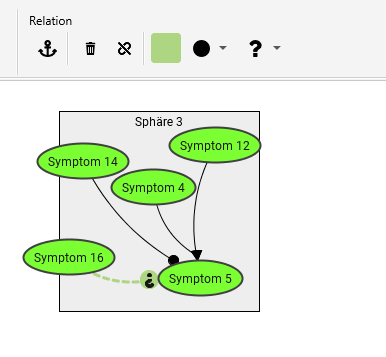
\includegraphics[width=0.4\columnwidth, keepaspectratio]{edge.png} 
			}		
			\caption{Relationen}	
		\end{figure}
		
%%%%%%%%%%%%%%%%%%%%%%%%%%%%%%%%%%%%%%%%%%%%%%%%%%%%%%%%%%%%%%%%%%%%%%%%%%%%%%%%%%%%%%%%%%%%%%%%%%%%%%%%%%%%%
		\subsubsection{Relation entfernen}
		\condition
		Es muss mindestens eine Relation in dem Syndrom existieren. 
		\actions
		\aOne
		\begin{enumerate}
			\item Die Relation, die gelöscht werden soll mit einem Links-Klick auswählen.
			\item Die \textit{Entfernen}-Taste auf der Tastatur drücken.
		\end{enumerate}
		\aTwo
		\begin{enumerate}
			\item Die Relation, welche gelöscht werden soll mit einem Links-Klick auswählen.
			\item In der Menüleiste einen Links-Klick auf den Button \textit{Relation entfernen} ausführen.
		\end{enumerate}
		\aThree
		\begin{enumerate}
			\item Mit einem Rechts-Klick auf die Relation, welche gelöscht werden soll, das Kontextmenü öffnen. 
			\item In diesem Kontextmenü die \textit{Entfernen}-Option mit einem Links-Klick auswählen. \\
		\end{enumerate}
		
%%%%%%%%%%%%%%%%%%%%%%%%%%%%%%%%%%%%%%%%%%%%%%%%%%%%%%%%%%%%%%%%%%%%%%%%%%%%%%%%%%%%%%%%%%%%%%%%%%%%%%%%%%%%%
\subsubsection{Ankerpunkte ein-/ ausblenden}
		Ankerpunkte bezeichnen die Postion, wo die Relation in einem Symptom mündet/ von ihm ausgeht. Bei der Erstellung einer Relation werden diese automatisch gesetzt und sind veränderbar. Das bedeutet, dass wenn ein Symptom bewegt wird, sich die Postion der Mündung/Ausgang der Relation in/aus das Symptom entsprechend anpasst und bewegt. Um das zu verhindert, können die Ankerpunkte manuell gesetzt werden. Diese sind dann fest, d.h. auch beim Bewegen eines Symptoms bleibt die Position der Mündung/ des Ausgangs bestehen.
		\condition
		Es muss mindestens eine Relation im Syndromansatz existieren und mindestens ein Ankerpunkt gesetzt sein. 
		\action
		\begin{enumerate}
			\item In der Menüleiste den Button \textit{Ankerpunkte ein-/ausblenden} durch einen Links- Klick aktivieren.
			\item Zum Ausblenden den Button durch einen Links- Klick deaktivieren. 
		\end{enumerate}
		\hint
		\begin{itemize}
			\item Die Ankerpunkte werden beim Einblenden rot eingefärbt. 
		\end{itemize}
		\begin{figure}[ht!]
			\centering
			\subfigure{
				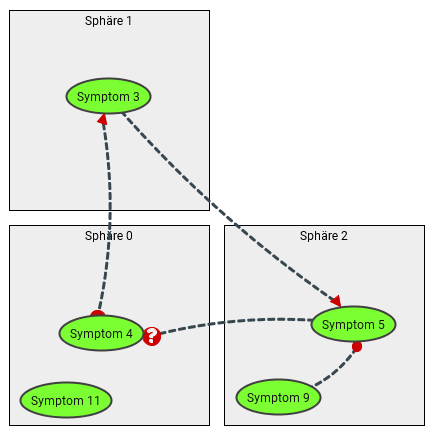
\includegraphics[width=0.4\columnwidth, keepaspectratio]{anchor.png} 
			}	
			\caption{Ankerpunkte}		
		\end{figure}
		
		\newpage
%%%%%%%%%%%%%%%%%%%%%%%%%%%%%%%%%%%%%%%%%%%%%%%%%%%%%%%%%%%%%%%%%%%%%%%%%%%%%%%%%%%%%%%%%%%%%%%%%%%%%%%%%%%%%	
\subsubsection{Ankerpunkte hinzufügen}
		\condition
		Es muss mindestens eine Relation im Syndromansatz existieren.
		\action
		\begin{enumerate}
			\item Die Kante durch einen Rechts- Klick auswählen und gedrückt halten.
			\item Befindet sich die Position der Maus beim Klick näher am Symptom, in welches die Relation mündet, wird der Ankerpunkt der Mündung der Relation gesetzt. Befindet sich die Position der Maus beim Klick näher am Symptom, von dem die Kante ausgeht, wird der Ankerpunkt für den Ausgang der Kante gesetzt. 
			\item Die Kante in die gewünschte Richtung bewegen. Die Mündung/ der Ausgang der Kante wandert entsprechend mit. 
			\item Wenn die gewünschte Position erreicht ist, die gedrückte Maustaste loslassen. 
		\end{enumerate}
		\begin{figure}[ht!]
			\centering
			\subfigure{
				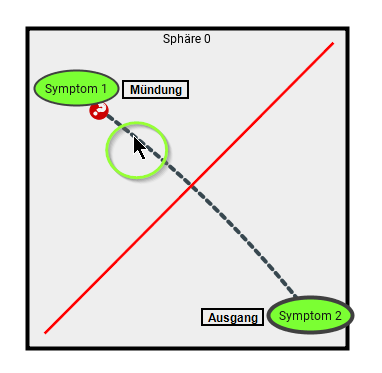
\includegraphics[width=0.3\columnwidth, keepaspectratio]{add_anchor.png} 
			}	
			\caption{Ankerpunkt hinzufügen}		
		\end{figure}
		\hint
		\begin{itemize}
			\item Beim Beispiel in der Abbildung wird aufgrund der Mausposition der Ankerpunkt bei der Mündung der Relation gesetzt. \\
		\end{itemize}
		
%%%%%%%%%%%%%%%%%%%%%%%%%%%%%%%%%%%%%%%%%%%%%%%%%%%%%%%%%%%%%%%%%%%%%%%%%%%%%%%%%%%%%%%%%%%%%%%%%%%%%%%%%%%%%
\subsubsection{Ankerpunkte entfernen}
		\condition
		Es muss mindestens eine Relation im Syndromansatz existieren.
		\action
		\begin{enumerate}
			\item Die gewünschte Relation durch einen Link- Klick auswählen. 
			\item In der Menüleiste einen Links-Klick auf den Button \textit{Ankerpunkt entfernen} ausführen.
		\end{enumerate}
		\hint
		\begin{itemize}
			\item Beim Entfernen der Ankerpunkte werden immer (wenn gesetzt) beide Ankerpunkte entfernt.\\
		\end{itemize}
		
%%%%%%%%%%%%%%%%%%%%%%%%%%%%%%%%%%%%%%%%%%%%%%%%%%%%%%%%%%%%%%%%%%%%%%%%%%%%%%%%%%%%%%%%%%%%%%%%%%%%%%%%%%%%%
\subsubsection{Farbe einer Relation verändern}
		\condition
		Es muss mindestens eine Relation im Syndromansatz existieren.
		\actions
		\aOne
		\begin{enumerate}
			\item In der Menüleiste mit der linken Maustaste auf den Button \textit{Farbe der Relation verändern} klicken.
			\item Mit einem Rechts-Klick auf die Relation, deren Farbe geändert werden soll, das Kontextmenü öffnen.
			\item Im Kontextmenü den Punkt \textit{Relationsfarbe} auswählen.
		\end{enumerate}
		\aTwo
		\begin{enumerate}
			\item Die Relation, deren Farbe geändert werden soll, mit einem Links-Klick auswählen.
			\item In der Menüleiste mit der linken Maustaste einen Links-Klick auf den Button \textit{Farbe der Relation verändern} ausführen.
			\item In dem sich öffnenden Fenster die gewünschte Farbe mit einem auswählen. \\
		\end{enumerate}	
		
%%%%%%%%%%%%%%%%%%%%%%%%%%%%%%%%%%%%%%%%%%%%%%%%%%%%%%%%%%%%%%%%%%%%%%%%%%%%%%%%%%%%%%%%%%%%%%%%%%%%%%%%%%%%%
\subsubsection{Type einer Relation verändern}
		\condition
		Es muss mindestens eine Relation im Syndromansatz existieren.
		\actions
		\aOne
		\begin{enumerate}
			\item In der Menüleiste mit der linken Maustaste auf den Button \textit{Typ der Relation verändern} klicken.
			\item Aus dem Drop-Down-Menü den gewünschten Typ per Links- Klick auswählen.
			\item Mit einem Rechts-Klick auf die Relation, deren Typ geändert werden soll, das Kontextmenü öffnen.
			\item Im Kontextmenü den Punkt \textit{Typ} auswählen.
		\end{enumerate}
		\aTwo
		\begin{enumerate}
			\item Die Relation, deren Typ geändert werden soll, mit einem Links-Klick auswählen.
			\item In der Menüleiste mit der linken Maustaste einen Links-Klick auf den Button \textit{Typ der Relation verändern} ausführen.
			\item Aus dem Drop-Down einen Typ per Links- Klick auswählen. 
		\end{enumerate}	
		\hint
		\begin{itemize}
			\item Die normale Pfeilspitze stellt die verstärkende Beziehung von Relationen im Syndromansatz dar.
			\item Die kreisförmige Pfeilspitze stellt die abschwächend Beziehung von Relationen im Syndromansatz dar.
			\item Die Pfeilspitze mit dem Fragezeichen stellt die neutrale Beziehung von Relationen im Syndromansatz dar.
		\end{itemize}
		
%%%%%%%%%%%%%%%%%%%%%%%%%%%%%%%%%%%%%%%%%%%%%%%%%%%%%%%%%%%%%%%%%%%%%%%%%%%%%%%%%%%%%%%%%%%%%%%%%%%%%%%%%%%%%
		\subsubsection{Graphelemente zu der Hervorhebung hinzufügen}
		\condition 	
		Ein Syndrom mit mindestens einer Sphäre, die ein oder mehr Symptome und eine oder mehr Relationen enthält, ist im Programm geöffnet. 
		\actions
		\aOne
		\begin{enumerate}
			\item Das Symptom/ die Relation, welche(s) hervorgehoben werden soll, mit einem Links-Klick auswählen. 
			\item In der Menüleiste den Button \textit{Elemente hervorheben} klicken.
		\end{enumerate}
		\aTwo
		\begin{enumerate}
			\item Im Kontextmenü des Graphelements, das hervorgehoben werden soll, die Option \textit{Hervorhebung} mit einem Links-Klick auswählen.
		\end{enumerate}
		\hint
		\begin{itemize}
					\item Es können lediglich Symptome und Relationen hervorgehoben werden.
					\item Wird die Aktion auf einem Graphelement ausgeführt, das aktuell bereits hervorgehoben ist, passiert nichts.
					\item Um die Hervorhebung zu aktivieren/ sichtbar zu machen den Button \textit{Hervorgehobene Elemente aktivieren} in der Menüleiste anklicken. Durch einen erneuten Klick auf diesen Button wird die Hervorhebung wieder deaktiviert. Dabei kann dieser \textit{Hervorgehobene Elemente aktivieren}-Button zu einem beliebigen Zeitpunkt im oben beschriebenen Ablauf geklickt werden.
					\item Ist die Hervorhebung durch den \textit{Hervorgehobene Elemente aktivieren}-Button momentan nicht aktiv hat diese Aktion keine visuellen Effekt. 
					\item Im Kontextmenü wird die Option \textit{Hervorhebung} farblich hervorgehoben, falls das Element schon der \textit{Hervorhebung} hinzugefügt wurde. \\
		\end{itemize}
			
%%%%%%%%%%%%%%%%%%%%%%%%%%%%%%%%%%%%%%%%%%%%%%%%%%%%%%%%%%%%%%%%%%%%%%%%%%%%%%%%%%%%%%%%%%%%%%%%%%%%%%%%%%%%
\subsubsection{Graphelemente aus der Hervorhebung entfernen}
		\condition 	
		Ein Syndrom mit mindestens einer Sphäre, die ein oder mehr Symptome und eine oder mehr Relationen enthält, ist im Programm geöffnet. Es ist mindestens eines dieser Elemente hervorgehoben.
		\actions
		\aOne
		\begin{enumerate}
			\item Das Symptom/ die Relation, welche(s) aktuell hervorgehoben ist und deren Hervorhebung aufgehoben werden soll, mit einem Links-Klick auswählen. 
			\item In der Menüleiste den Button \textit{Hervorhebung von Elementen entfernen} klicken.
		\end{enumerate}
		\aTwo
		\begin{enumerate}
			\item Im Kontextmenü des Graphelements, das aktuell hervorgehoben ist und dessen Hervorhebung aufgehoben werden soll, die Option \textit{Hervorhebung} mit einem Links-Klick auswählen.
		\end{enumerate}
		\hint
		\begin{itemize}
			\item Wird die Aktion auf einem Graphelement ausgeführt, das aktuell nicht hervorgehoben ist, passiert nichts.
			\item Die bereits hervorgehoben Elemente, die nicht vor Klicken des \textit{Hervorhebung von Elementen entfernen}-Buttons ausgewählt wurden, bleiben hervorgehoben.
			\item Im Kontextmenü von hervorgehobenen Elementen wird der Option \textit{Hervorhebung}  farblich hervorgehoben angezeigt, was verdeutlicht, dass dieses Element aktuell hervorgehoben ist und dass ein erneutes Klicken auf diese Schaltfläche die Hervorhebung aufhebt. \\
		\end{itemize}
	
%%%%%%%%%%%%%%%%%%%%%%%%%%%%%%%%%%%%%%%%%%%%%%%%%%%%%%%%%%%%%%%%%%%%%%%%%%%%%%%%%%%%%%%%%%%%%%%%%%%%%%%%%%%%%%%%%%%%%
\subsection{Hervorhebung aktivieren/ deaktivieren}

\begin{figure}[ht!]
	\centering
	\subfigure[Hervorhebung]{
		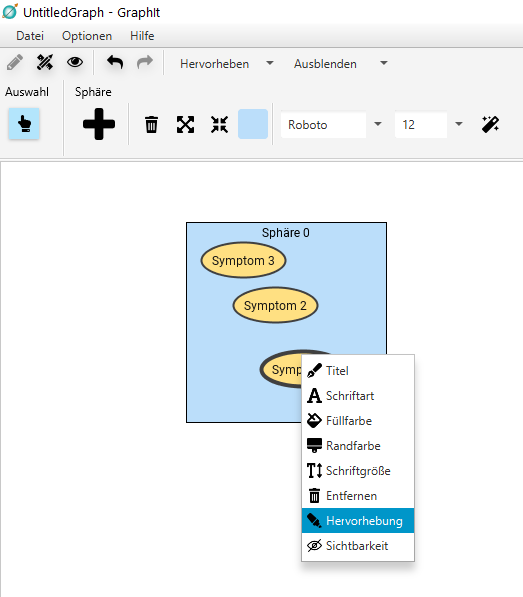
\includegraphics[width=0.4\columnwidth, keepaspectratio]{highlight2.png} 
	}
	\subfigure[Hervorhebung(2)]{
		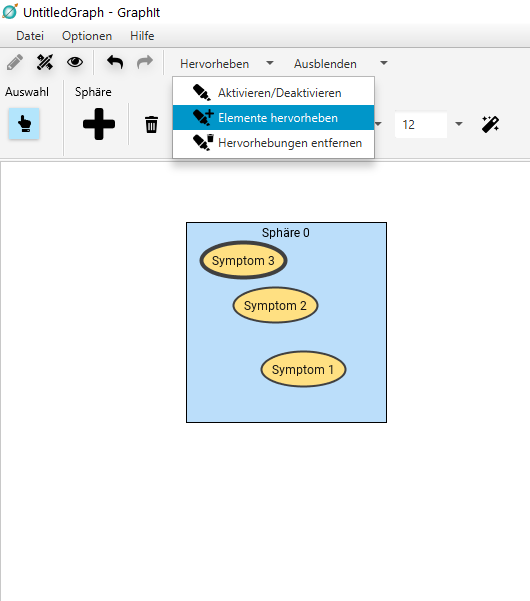
\includegraphics[width=0.4\columnwidth, keepaspectratio]{highlight.png} 
	}
	\caption{Hervorhebung}
	
\end{figure}

%%%%%%%%%%%%%%%%%%%%%%%%%%%%%%%%%%%%%%%%%%%%%%%%%%%%%%%%%%%%%%%%%%%%%%%%%%%%%%%%%%%%%%%%%%%%%%%%%%%%%%%%%%%%%	
\subsubsection{Graphelemente ausblenden/einblenden}
		\condition 	
		Ein Syndrom mit mindestens einer Sphäre, die ein oder mehr Symptome und beliebig viele Relationen enthält, ist im Programm geöffnet.
		\action
			\begin{enumerate}
				\item In der Menüleiste den Button \textit{Ausgeblendete Elemente aktivieren} mit einem Links-Klick aktivieren.
			\end{enumerate}
		\hint
		\begin{itemize}
				\item Die als ausgeblendet eingestellten Elemente werden (visuell) ausgeblendet. 
				\item Die ausgeblendeten Elemente sind weiterhin im Graphen enthalten und können jeder Zeit wieder eingeblendet werden. 
				\item Ist ein Symptom als ausgeblendet eingestellt und wird der \textit{Ausgeblendete Elemente aktivieren}-Button aktiviert, so werden auch die Relationen, die zu diesem Symptom hinführen und von diesem ausgehen ausgeblendet. Sie werden zusammen mit dem Symptom beim erneuten Klicken dieses Buttons wieder eingeblendet.
				\item Durch erneutes Klicken des \textit{Ausgeblendete Elemente aktivieren}-Buttons wird die (visuelle) Ausblendung der Elemente aufgehoben. \\
		\end{itemize}
		
%%%%%%%%%%%%%%%%%%%%%%%%%%%%%%%%%%%%%%%%%%%%%%%%%%%%%%%%%%%%%%%%%%%%%%%%%%%%%%%%%%%%%%%%%%%%%%%%%%%%%%%%%%%%%
\subsubsection{Graphelemente zum Fadeout hinzufügen}
	\condition 	
		Ein Syndrom mit mindestens einer Sphäre, die ein oder mehr Symptome und beliebig viele Relationen enthält, ist im Programm geöffnet. 
		\actions
		\aOne
		\begin{enumerate}
			\item Das Symptom / die Relation, welche(s) ausgeblendet werden soll, mit einem Links-Klick auswählen. 
			\item In der Menüleiste den Button \textit{Elemente ausblenden} klicken.
		\end{enumerate}
		\aTwo
		\begin{enumerate}
			\item Im Kontextmenü des Graphelements, das ausgeblendet werden soll, die Option \textit{Sichtbarkeit} mit einem Links-Klick auswählen.
		\end{enumerate}
		\hint
		\begin{itemize}
					\item Es können lediglich Symptome und Relationen ausgeblendet werden. 
					\item Wird ein Symptom ausgeblendet, so auch die Relationen, die zu/von diesem Symptom führen/ ausgehen.
					\item Wird die Aktion auf einem Graphelement ausgeführt, das aktuell bereits als ausgeblendet ist, passiert nichts.
					\item Um die Ausblendung zu aktivieren/ sichtbar zu machen den Button \textit{Ausgeblendete Elemente aktivieren} in der Menüleiste anklicken. Durch einen erneuten Klick auf diesen Button wird die Ausblendung wieder deaktiviert. Dabei kann dieser \textit{Ausgeblendete Elemente aktivieren}-Button zu einem beliebigen Zeitpunkt im oben beschriebenen Ablauf geklickt werden.
					\item Fall ein Graphelement bereits dem Fadeout hinzugefügt wurde, wird die Option \textit{Sichtbarkeit} im Kontextmenü des Elementes farblich hervorgehoben. \\
		\end{itemize}
		
%%%%%%%%%%%%%%%%%%%%%%%%%%%%%%%%%%%%%%%%%%%%%%%%%%%%%%%%%%%%%%%%%%%%%%%%%%%%%%%%%%%%%%%%%%%%%%%%%%%%%%%%%%%%%
\subsubsection{Graphelemente aus dem Fadeout entfernen}
		\condition 	
		Ein Syndrom mit mindestens einer Sphäre, die ein oder mehr Symptome und beliebig viele Relationen enthält, ist im Programm geöffnet. Es ist mindestens eines dieser Elemente als ausgeblendet eingestellt.
		\actions
		\aOne
		\begin{enumerate}
			\item Das Symptom/ die Relation, welche(s) aktuell als ausgeblendet eingestellt ist und dessen/ deren Ausblendung aufgehoben werden soll, mit einem Links-Klick auswählen. 
			\item In der Menüleiste den Button \textit{Ausblendung von Elementen entfernen} klicken.
		\end{enumerate}
		\aTwo
		\begin{enumerate}
			\item Im Kontextmenü des Graphelements, das aktuell als ausgeblendet eingestellt ist und dessen Ausblendung aufgehoben werden soll, die Option \textit{Sichtbarkeit} mit einem Links-Klick auswählen.
		\end{enumerate}
		\hint
		\begin{itemize}
				\item Wird die Aktion auf einem Graphelement ausgeführt, das aktuell nicht ausgeblendet ist, passiert nichts.
				\item Im Kontextmenü von als ausgeblendet eingestellten Elementen wird die Option \textit{Sichtbarkeit} farblich hervorgehoben, was verdeutlicht, dass dieses Element aktuell als ausgeblendet eingestellt ist und dass ein erneutes Klicken auf diese Schaltfläche die Ausblendung aufhebt.\\
		\end{itemize}	
		
%%%%%%%%%%%%%%%%%%%%%%%%%%%%%%%%%%%%%%%%%%%%%%%%%%%%%%%%%%%%%%%%%%%%%%%%%%%%%%%%%%%%%%%
\subsection{Zoom} \label{zoom}
		\subsubsection{Zoom}
		\condition 	
		Das Programm ist geöffnet.
		\actions
		\aOne
		\begin{enumerate}
			\item Das Zoom Fenster und der Zoom Slider befinden sich in der rechten unteren Ecke der Benutzeroberfläche.
			\item Links neben dem Zoom Slider auf die Anzeige der Prozent-Zahl einen Links-Klick ausführen (Bei Programmstart ist der Zoom auf 100\% eingestellt). 
			\item In dem sich öffnenden Menü eine der angebotenen Prozentzahlen mit einem Links-Klick auswählen.
		\end{enumerate}
		\aTwo
		\begin{enumerate}
			\item Den Schieber auf den Zoom Slider durch einen Links-Klick auswählen und die Maustaste gedrückt halten. 
			\item Zum Vergrößern der Darstellung des Syndroms nach rechts und zum Verkleinern in der Leiste nach links schieben.
			\item Den Button bei Erreichen der gewünschten Größe loslassen.
		\end{enumerate}
		\hint
		\begin{itemize}
			\item Der Zoom- Bereich liegt zwischen 20 und 200 \%.
	 	\end{itemize}		

\newpage	
%%%%%%%%%%%%%%%%%%%%%%%%%%%%%%%%%%%%%%%%%%%%%%%%%%%%%%%%%%%%%%%%%%%%%%%%%%%%%%%%%%%%%%%
		\subsubsection{Zoom Fenster}
		\condition 	
		Das Programm ist geöffnet.
		\action
		\begin{enumerate}
				\item Den Cursor in das Zoom Fenster in der Anwendung bewegen und dort die linke Maustaste drücken.
				\item Die linke Maustaste gedrückt halten und den Cursor innerhalb des Übersichtsfensters verschieben.
				\item Die linke Maustaste loslassen, sobald im Hauptfenster der gewünschte Bereich angezeigt wird.
		\end{enumerate}
		\hint
		\begin{itemize}
				\item Das weiße Feld innerhalb des Zoom Fensters stellt den Ausschnitt des aktuell im Hauptfenster angezeigten Syndroms dar.
				\item Falls Teile des erstellten Syndroms nicht im Hauptfenster sichtbar sind, kann es sein, dass sich diese nicht in dem aktuell angezeigten Bereich befinden. Durch heraus zoomen werden diese wahrscheinlich wieder angezeigt.  
	 	\end{itemize}
 	
 		\begin{figure}[ht!]
 			\centering
 			\subfigure[Zoom Slider]{
 				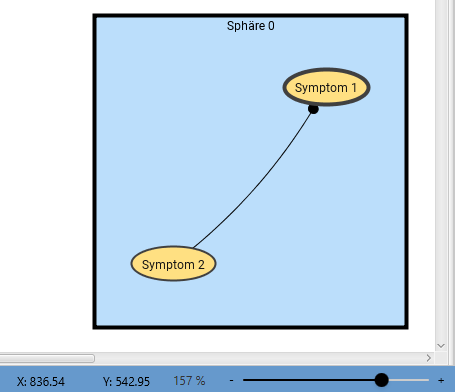
\includegraphics[width=0.4\columnwidth, keepaspectratio]{zoom_slider.png} 
 			}
 			\subfigure[Zoom Fenster]{
 				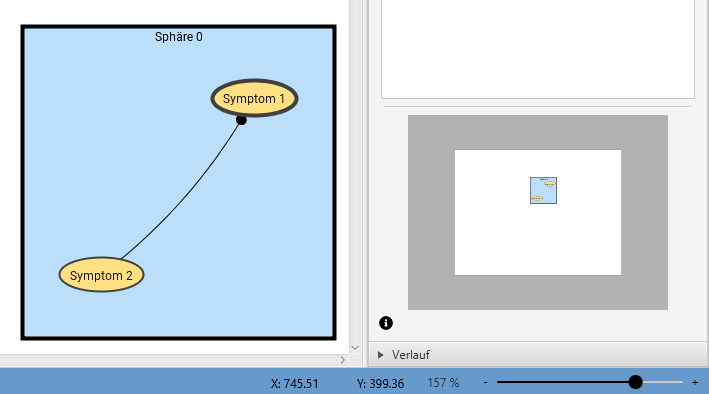
\includegraphics[width=0.4\columnwidth, keepaspectratio]{zoom_window.png} 
 			}
 			\caption{Zoom}
 		\end{figure}
%%%%%%%%%%%%%%%%%%%%%%%%%%%%%%%%%%%%%%%%%%%%%%%%%%%%%%%%%%%%%%%%%%%%%%%%%%%%%%%%%%%%%%%%%%%%%%%			
		
\subsection{Allgemeine Einstellungen} \label{settings}
	
\subsection{Sprache}
\textbf{GraphIt} unterstützt die Sprachen Deutsch und Englisch. Dies betrifft sowohl die Elemente auf der Benutzeroberfläche (Buttons, Infotexte etc.) als auch die Beschriftung von den Elementen des Syndroms (Titel von Sphären und Symptomen).\\
	
\newpage
%%%%%%%%%%%%%%%%%%%%%%%%%%%%%%%%%%%%%%%%%%%%%%%%%%%%%%%%%%%%%%%%%%%%%%%%%%%%%%%%%%%%%%%
\subsubsection{Sprache der Benutzeroberfläche und der Graphelemente}
		\condition 	
		Das Programm ist geöffnet.
		\action
		\begin{enumerate}
				\item In der obersten Menüleiste auf \textit{Optionen} klicken. 
				\item In dem sich öffnenden Drop-Down-Menü den Cursor auf die Option \textit{Sprache} bewegen.
				\item Den Cursor auf Höhe dieser Schaltfläche in das Folgemenü bewegen, in dem \textit{Deutsch}/ \textit{Englisch} angezeigt wird.
				\item Die gewünschte Sprache in diesem Menü mit einem Links-Klick auswählen.\\
		\end{enumerate}

%%%%%%%%%%%%%%%%%%%%%%%%%%%%%%%%%%%%%%%%%%%%%%%%%%%%%%%%%%%%%%%%%%%%%%%%%%%%%%%%%%%%%%%	 		
\subsubsection{Sprache der Benutzeroberfläche}
		\condition 	
		Das Programm ist geöffnet.
		\action
		\begin{enumerate}
				\item In der obersten Menüleiste auf \textit{Optionen} klicken 
				\item In dem sich öffnenden Drop-Down-Menü den Cursor auf die Option \textit{Erweiterte Spracheinstellungen} bewegen.
				\item Den Cursor auf Höhe dieser Schaltfläche in das Folgemenü bewegen, in die Optionen \textit{Sprache der Benutzeroberfläche} und \textit{Sprache des Graphen} angezeigt wird.
				\item Den Cursor auf Höhe der Schaltfläche \textit{Sprache der Benutzeroberfläche} in das Folgemenü bewegen, in dem \textit{Deutsch}/ \textit{Englisch} angezeigt wird.
				\item Die gewünschte Sprache in diesem Menü mit einem Links-Klick auswählen. \\
		\end{enumerate}
	 		
%%%%%%%%%%%%%%%%%%%%%%%%%%%%%%%%%%%%%%%%%%%%%%%%%%%%%%%%%%%%%%%%%%%%%%%%%%%%%%%%%%%%%%%
\subsubsection{Sprache der Beschriftung der Graphelement}
		\condition 	
		Das Programm ist geöffnet.
		\action
		\begin{enumerate}
				\item In der obersten Menüleiste auf \textit{Optionen} klicken 
				\item In dem sich öffnenden Drop-Down-Menü den Cursor auf die Option \textit{Erweiterte Spracheinstellungen} bewegen.
				\item Den Cursor auf Höhe dieser Schaltfläche in das Folgemenü bewegen, in die Optionen \textit{Sprache der Benutzeroberfläche} und \textit{Sprache des Graphen} angezeigt wird.
				\item Den Cursor auf Höhe der Schaltfläche \textit{Sprache des Graphen} in das Folgemenü bewegen, in dem \textit{Deutsch}/ \textit{Englisch} angezeigt wird.
				\item Die gewünschte Sprache in diesem Menü mit einem Links-Klick auswählen.
		\end{enumerate}
	 	
%%%%%%%%%%%%%%%%%%%%%%%%%%%%%%%%%%%%%%%%%%%%%%%%%%%%%%%%%%%%%%%%%%%%%%%%%%%%%%%%%%%%%%%
\subsection{Dateiformate für den Export/Import/ und das Speichern/Öffnen} 
Das Exportieren und Speichern ist dazu gedacht, Daten auch außerhalb der Anwendung sichern zu können. Diese Daten können zu einem späteren Zeitpunkt wieder in \textbf{GraphIt} geladen werden, in dem die entsprechenden Dateien wieder importiert/ geöffnet werden.\\
In \textbf{GraphIt} sind dabei die folgenden Datei-Formate von Relevanz: 
\begin{itemize}
\item .oof-Format
\item .gxl-Format
\item .txt-Format
\item .pdf-Format
\end{itemize}

	\subsubsection{OOF}
	Dieses Datei-Format dient der gemeinsamen Speicherung des Protokolls der Nutzerinteraktionen und eines Syndroms. Somit kann beispielsweise ein Bearbeiter sein erstelltes Syndrom zusammen mit den dabei aufgezeichneten Nutzerinteraktionen exportieren. Diese .oof- Datei kann nun von einem anderen Benutzer (beispielsweise einem Auswerter) importiert werden. .oof ist das Standardformat von \textbf{GraphIt}.
	
	\subsubsection{GXL}
	Dieses Datei-Format (\texttt{G}raph e\texttt{X}change \texttt{L}anguage) dient der Speicherung vom Graphen außerhalb der Anwendung. Die gespeicherte Datei kann entweder lediglich eine Beschreibung des Graphen als solchen in GXL-Notation beinhalten oder zusätzlich Informationen zu den Vorlage-Regeln speichern. Dies ermöglicht es, einen Graphen zu erstellen und diesen zu einem späteren Zeitpunkt auf dem selben oder auch einem anderen Computer wieder in \textbf{GraphIt} zu laden. Letzteres ist insbesondere dann von Nutzen, wenn ein Graph mit Regeln für die Bearbeitung erstellt wurde und im Anschluss von anderen Personen gemäß der Vorlageregeln bearbeitet werden soll.
	
	\subsubsection{Textdatei (TXT)}
	Dieses Format dient dazu ein Protokoll der Nutzerinteraktionen zu exportieren. Dies ermöglicht es, den Erstellungsprozess eines Syndroms im Nachhinein analysieren zu können. Diese Datei ist nicht wieder von dem System importierbar. 
	
	\subsubsection{PDF}
	Dieses Format dient dazu, die Visualisierung eines Syndroms außerhalb der Anwendung sichern zu können. Mit diesem Format kann die ein Syndrom in seiner visualisierten Form auch außerhalb des System (zum Beispiel in einem Webbrowser) betrachtet werden. 
	
\newpage	
%%%%%%%%%%%%%%%%%%%%%%%%%%%%%%%%%%%%%%%%%%%%%%%%%%%%%%%%%%%%%%%%%%%%%%%%%%%%%%%%%%%%%%%
\subsection{Neue Datei/ Öffnen/ Importieren} \label{import}
	
\subsubsection{Neue Datei}
		\condition 	
		Das Programm ist geöffnet.
		\actions
		\aOne
		\begin{enumerate}
				\item Die \textit{Ctrl}-Taste der Tastatur drücken.
				\item Die Taste gedrückt halten und dabei zusätzlich die \textit{N}-Taste der Tastatur drücken.
		\end{enumerate}				
		\aTwo
		\begin{enumerate}
				\item In der obersten Menüleiste auf die Option \textit{Datei} klicken 
				\item In dem sich öffnenden Drop-Down-Menü den Cursor auf die Option \textit{Neue Datei} bewegen und mit einem Links-Klick bestätigen.
		\end{enumerate}		
		\hint
		\begin{itemize}
				\item Es erscheint ein Fenster, in dem die Aktion mit einem Links-Klick auf \textit{Weiter} bestätigt werden muss, wenn tatsächliche eine neue Datei erstellt werden soll. Mit einem Klick auf \textit{Abbrechen} wird keine neue Datei erstellt und das aktuell angezeigte Syndrom (sofern vorhanden) bleibt erhalten.
				\item Wird eine neue Datei erstellt, wird falls ein Syndrom derzeit im System geladen ist, dieses gelöscht und die Daten gehen verloren und können auch nicht wieder hergestellt werden. \\
		\end{itemize}
		
						
%%%%%%%%%%%%%%%%%%%%%%%%%%%%%%%%%%%%%%%%%%%%%%%%%%%%%%%%%%%%%%%%%%%%%%%%%%%%%%%%%%%%%%%
\subsubsection{Datei öffnen}
		\condition 	
		Das Programm ist geöffnet.
		\actions
		\aOne
		\begin{enumerate}
				\item Die \textit{Ctrl}-Taste der Tastatur drücken.
				\item Die Taste gedrückt halten und dabei zusätzlich die \textit{O}-Taste der Tastatur drücken.
		\end{enumerate}				
		\aTwo
		\begin{enumerate}
				\item In der obersten Menüleiste die Option \textit{Datei} auswählen. 
				\item In dem sich öffnenden Drop-Down-Menü den Cursor auf die Option \textit{Datei öffnen} bewegen und mit einem Links-Klick bestätigen.
		\end{enumerate}		
		\hint
		\begin{itemize}
				\item Es erscheint ein Fenster, in dem die Aktion mit einem Links-Klick auf \textit{Weiter} bestätigt werden muss, wenn tatsächliche eine Datei geöffnet werden soll. Mit einem Klick auf \textit{Abbrechen} wird keine Datei geöffnet und das aktuell angezeigte Syndrom (sofern vorhanden) bleibt erhalten.
				\item  Wird eine Datei geöffnet, wird falls ein Syndrom derzeit im System geladen ist, dieses gelöscht und die Daten gehen verloren und können auch nicht wieder hergestellt werden. 
				\item \textit{Datei öffnen} entspricht dem Vorgang eine .oof- Datei zu importieren. \\
		\end{itemize}

%%%%%%%%%%%%%%%%%%%%%%%%%%%%%%%%%%%%%%%%%%%%%%%%%%%%%%%%%%%%%%%%%%%%%%%%%%%%%%%%%%%%%%%
\subsubsection{Importieren als  Vorlage}
		\condition 	
		Das Programm ist geöffnet.
		\actions
		\aOne
		\begin{enumerate}
				\item Die \textit{Ctrl}-Taste der Tastatur drücken.
				\item Die Taste gedrückt halten und dabei zusätzlich die \textit{I}-Taste der Tastatur drücken.
		\end{enumerate}				
		\aTwo
		\begin{enumerate}
				\item In der obersten Menüleiste die Option \textit{Datei} auswählen. 
				\item In dem sich öffnenden Drop-Down-Menü den Cursor auf die Option \textit{Importieren als...} bewegen.
				\item Auf der Höhe dieser Schaltfläche den Cursor in das sich öffnende Menü bewegen, das die Optionen \textit{Vorlage} und \textit{GXL} enthält.
				\item In diesem Menü die Option \textit{Vorlage} mit einem Links-Klick auswählen.
		\end{enumerate}		
		\hint
		\begin{itemize}
				\item Bei dieser Variante des Imports wird ein Graph mit den Vorlageregeln importiert.
				\item Es erscheint ein Fenster, in dem die Aktion mit einem Links-Klick auf \textit{Weiter} bestätigt werden muss, wenn tatsächliche eine Datei importiert werden soll. Mit einem Klick auf \textit{Abbrechen} wird keine Datei importiert und das aktuell angezeigte Syndrom (sofern vorhanden) bleibt erhalten.
				\item  Wird eine Datei geöffnet, wird falls ein Syndrom derzeit im System geladen ist, dieses gelöscht und die Daten gehen verloren und können auch nicht wieder hergestellt werden. \\ 
		\end{itemize}

%%%%%%%%%%%%%%%%%%%%%%%%%%%%%%%%%%%%%%%%%%%%%%%%%%%%%%%%%%%%%%%%%%%%%%%%%%%%%%%%%%%%%%%
	\subsubsection{Importieren als GXL}
		\condition 	
		Das Programm ist geöffnet.
		\actions
		\aOne
		\begin{enumerate}
				\item Die \textit{Ctrl}-Taste der Tastatur drücken und gedrückt halten.
				\item Zusätzlich die \textit{Shift}-Taste drücken und ebenfalls gedrückt halten.
				\item Die beiden Tasten gedrückt halten und dabei zusätzlich die \textit{I}-Taste der Tastatur drücken.
		\end{enumerate}				
		\aTwo
		\begin{enumerate}
				\item In der obersten Menüleiste die Option \textit{Datei} auswählen. 
				\item In dem sich öffnenden Drop-Down-Menü den Cursor auf die Option \textit{Importieren als...} bewegen.
				\item Auf der Höhe dieser Schaltfläche den Cursor in das sich öffnende Menü bewegen, das die Optionen \textit{Vorlage} und \textit{GXL} enthält.
				\item In diesem Menü die Option \textit{GXL} mit einem Links-Klick auswählen.
		\end{enumerate}		
		\hint
		\begin{itemize}
				\item Bei dieser Variante des Imports wird ein Graph ohne Bearbeitungsregeln importiert, selbst wenn in der importierten Datei Bearbeitungsregeln gesetzt sind.
				\item Es erscheint ein Fenster, in dem die Aktion mit einem Links-Klick auf \textit{Weiter} bestätigt werden muss, wenn tatsächliche eine Datei importiert werden soll. Mit einem Klick auf \textit{Abbrechen} wird keine Datei importiert und das aktuell angezeigte Syndrom (sofern vorhanden) bleibt erhalten. \\
		\end{itemize}
		
%%%%%%%%%%%%%%%%%%%%%%%%%%%%%%%%%%%%%%%%%%%%%%%%%%%%%%%%%%%%%%%%%%%%%%%%%%%%%%%%%%%%%%%%%%%
\subsection{Speichern/ Exportieren} \label{export}

\subsubsection{Speichern unter}
		\condition 	
		Das Programm ist geöffnet.
		\actions
		\aOne
		\begin{enumerate}
				\item Die \textit{Ctrl}-Taste der Tastatur drücken.
				\item Die Taste gedrückt halten und dabei zusätzlich die \textit{S}-Taste der Tastatur drücken.
		\end{enumerate}				
		\aTwo
		\begin{enumerate}
				\item In der obersten Menüleiste die Option \textit{Datei} auswählen. 
				\item In dem sich öffnenden Drop-Down-Menü den Cursor auf die Option \textit{Speichern unter} bewegen und mit einem Links-Klick bestätigen.
		\end{enumerate}		
		\hint
		\begin{itemize}
				\item Bei den gespeicherten Daten handelt es sich sowohl um das Protokoll der Nutzerinteraktionen als auch um den aktuellen Graphen. Diese Informationen werden gemeinsam im .oof-Format (\textbf{GraphIt}s eigenes Datei-Format) gespeichert.\\
		\end{itemize}
		
%%%%%%%%%%%%%%%%%%%%%%%%%%%%%%%%%%%%%%%%%%%%%%%%%%%%%%%%%%%%%%%%%%%%%%%%%%%%%%%%%%%%
		\subsubsection{Exportieren als Vorlage}
		\condition 	
		Das Programm ist geöffnet.
		\actions
		\aOne
		\begin{enumerate}
				\item Die \textit{Ctrl}-Taste der Tastatur drücken und gedrückt halten.
				\item Zusätzlich die \textit{E}-Taste der Tastatur drücken.
		\end{enumerate}				
		\aTwo
		\begin{enumerate}
				\item In der obersten Menüleiste die Option \textit{Datei} auswählen. 
				\item In dem sich öffnenden Drop-Down-Menü den Cursor auf den die Option \textit{Exportieren als...} bewegen.
				\item Auf der Höhe dieser Schaltfläche den Cursor in das sich öffnende Menü bewegen, das die Optionen \textit{Vorlage}, \textit{GXL}, \textit{PDF} und \textit{Verlaufsprotokoll} beinhaltet.
				\item In diesem Menü die Option \textit{Vorlage} mit einem Links-Klick auswählen.
		\end{enumerate}		
		\hint
		\begin{itemize}
				\item Bei dieser Variante des Exports wird ein Graph mit den gesetzten Vorlageregeln exportiert. \\
		\end{itemize}
		
%%%%%%%%%%%%%%%%%%%%%%%%%%%%%%%%%%%%%%%%%%%%%%%%%%%%%%%%%%%%%%%%%%%%%%%%%%%%%%%%%%%%%%%
\subsubsection{Exportieren als GXL}
		\condition 	
		Das Programm ist geöffnet.
		\actions
		\aOne
		\begin{enumerate}
				\item Die \textit{Ctrl}-Taste der Tastatur drücken und gedrückt halten.
				\item Zusätzlich die \textit{Shift}-Taste drücken und ebenfalls gedrückt halten.
				\item Die beiden Tasten gedrückt halten und dabei zusätzlich die \textit{E}-Taste der Tastatur drücken.
		\end{enumerate}				
		\aTwo
		\begin{enumerate}
				\item In der obersten Menüleiste die Option \textit{Datei} auswählen. 
				\item In dem sich öffnenden Drop-Down-Menü den Cursor auf die Option \textit{Exportieren als...} bewegen.
				\item Auf der Höhe dieser Schaltfläche den Cursor in das sich öffnende Menü bewegen, das die Optionen \textit{Vorlage}, \textit{GXL}, \textit{PDF} und \textit{Verlaufsprotokoll} enthält.
				\item In diesem Menü die Option \textit{GXL} mit einem Links-Klick auswählen.
		\end{enumerate}		
		\hint
		\begin{itemize}
				\item Bei dieser Variante des Exports wird ein Graph ohne gesetzte Vorlageregeln exportiert (selbst wenn Regeln in der Anwendung eingegeben wurden). \\
		\end{itemize}
		
%%%%%%%%%%%%%%%%%%%%%%%%%%%%%%%%%%%%%%%%%%%%%%%%%%%%%%%%%%%%%%%%%%%%%%%%%%%%%%%%%%%%%%%
		\subsubsection{Exportieren als PDF}
		\condition 	
		Das Programm ist geöffnet.
		\actions
		\aOne
		\begin{enumerate}
				\item Die \textit{Ctrl}-Taste der Tastatur drücken und gedrückt halten.
				\item Zusätzlich die \textit{Shift}-Taste drücken und ebenfalls gedrückt halten.
				\item Die beiden Tasten gedrückt halten und dabei zusätzlich die \textit{P}-Taste der Tastatur drücken.
		\end{enumerate}				
		\aTwo
		\begin{enumerate}
				\item In der obersten Menüleiste die Option \textit{Datei} auswählen. 
				\item In dem sich öffnenden Drop-Down-Menü den Cursor auf die Option \textit{Exportieren als...} bewegen.
				\item Auf der Höhe dieser Schaltfläche den Cursor in das sich öffnende Menü bewegen, das die Optionen \textit{Vorlage}, \textit{GXL}, \textit{PDF} und \textit{Verlaufsprotokoll} enthält.
				\item In diesem Menü die Option \textit{PDF} mit einem Links-Klick auswählen.
		\end{enumerate}		
		\hint
		\begin{itemize}
				\item Bei dieser Variante des Exports wird die visuelle Darstellung eines Syndroms exportiert.
				\item Es erscheint ein Fenster, das darauf hinweist, dass nur der sichtbare Bereich des Syndroms als PDF exportiert wird. Durch Klicken auf \textit{Abbrechen} kann der Export-Vorgang abgebrochen werden. Klickt man auf \textit{Weiter} erscheint ein Fenster, in dem durch Navigation durch das Dateisystem der gewünschte Speicherort ausgewählt werden kann. \\
		\end{itemize}
		
%%%%%%%%%%%%%%%%%%%%%%%%%%%%%%%%%%%%%%%%%%%%%%%%%%%%%%%%%%%%%%%%%%%%%%%%%%%%%%%%%%%%%%%
\subsubsection{Exportieren des Verlaufsprotokolls}
		\condition 	
		Das Programm ist geöffnet.
		\actions
		\aOne
		\begin{enumerate}
				\item Die \textit{Ctrl}-Taste der Tastatur drücken und gedrückt halten.
				\item Zusätzlich die \textit{L}-Taste der Tastatur drücken.
		\end{enumerate}				
		\aTwo
		\begin{enumerate}
				\item In der obersten Menüleiste die Option \textit{Datei} auswählen. 
				\item In dem sich öffnenden Drop-Down-Menü den Cursor auf die Option \textit{Exportieren als...} bewegen.
				\item Auf der Höhe dieser Schaltfläche den Cursor in das sich öffnende Menü bewegen, das die Optionen \textit{Vorlage}, \textit{GXL}, \textit{PDF} und \textit{Verlaufsprotokoll} enthält.
				\item In diesem Menü die Option \textit{Verlaufsprotokoll} mit einem Links-Klick auswählen.
		\end{enumerate}		
		\hint
		\begin{itemize}
				\item Bei dieser Variante des Exports wird ein Protokoll der Nutzerinteraktionen in lesbarer Form exportiert. \\
		\end{itemize}

%%%%%%%%%%%%%%%%%%%%%%%%%%%%%%%%%%%%%%%%%%%%%%%%%%%%%%%%%%%%%%%%%%%%%%%%%%%%%%%%%%%%%%%%%%%%%%%%%%%%%%%%%%%%%%%%%%%
\subsection{Drucken} \label{print}
	\condition 
	Das Programm ist geöffnet.
	\actions
	\aOne
	\begin{enumerate}
		\item Einen Links-Klick in der obersten Menüleiste auf die Option \textit{Datei} aufführen.
		\item In dem sich öffnenden Drop-Down-Menü die Option \textit{Drucken} mit einem Links-Klick auswählen.
		\item Es erscheint ein Fenster, das darauf hinweist, dass nur der aktuell angezeigte/ sichtbare Teil des Syndroms gedruckt wird. In diesem Fenster auf den \textit{Weiter}-Button einen Links-Klick machen, um zum finalen Druckfenster zu gelangen. Auf den \textit{Abbrechen}-Button einen Links-Klick ausführen, wenn die Aktion abgebrochen werden soll.
		\item Wenn auf \textit{Weiter} geklickt wurde, erscheint das Fenster, in dem die Druckeinstellungen angepasst werden können. In diesem Fenster kann der Druckauftrag mit einem Links-Klick auf den \textit{OK}-Button abgeschickt oder die Aktion mit einem Links-Klick auf den \textit{Abbrechen}-Button aufgehoben werden.
	\end{enumerate} 
	\aTwo
	\begin{enumerate}
		\item Die \textit{Ctrl}-Taste drücken und gedrückt halten.
		\item Zusätzlich zur \textit{Ctrl}-Taste die \textit{P}-Taste betätigen.
		\item Es erscheint ein Fenster, das darauf hinweist, dass nur der aktuell angezeigte Teil des Syndroms gedruckt wird. In diesem Fenster auf den \textit{Weiter}-Button einen Links-Klick machen, um zum finalen Druckfenster zu gelangen. Auf den \textit{Abbrechen}-Button einen Links-Klick ausführen, wen die Aktion abgebrochen werden soll.
		\item Wenn auf \textit{Weiter} geklickt wurde, erscheint das Fenster, in dem die Druckeinstellungen angepasst werden können. In diesem Fenster kann der Druckauftrag mit einem Links-Klick auf den \textit{OK}-Button abgeschickt oder die Aktion mit einem Links-Klick auf den \textit{Abbrechen}-Button aufgehoben werden.
	\end{enumerate} 
	\hint
	\begin{itemize}
		\item Es wird nur der Bereich des Syndroms gedruckt, der gerade auch im Hauptfenster sichtbar ist.
		\item Die Druckeinstellungen erscheinen womöglich im Hintergrund, d.h. durch Bewegen der Maus auf das Icon von \textbf{GraphIt} in der Symbolleiste, kann durch Auswählen des dort erscheinenden Druckfensters dieses in den Vordergrund geholt werden. 
		\item Damit das Drucken funktioniert, muss auf dem Rechner ein Druckdienst installiert sein. Besonders wenn auf dem Betriebssystem Linux gearbeitet wird, bitte darauf achten. \\
	\end{itemize}

%%%%%%%%%%%%%%%%%%%%%%%%%%%%%%%%%%%%%%%%%%%%%%%%%%%%%%%%%%%%%%%%%%%%%%%%%%%%%%%%%%%%%%%%%%%%%%%%%%%%%%%%%%%%%%%%%%%
\subsection{Analysefunktionen} \label{analyse}
Die Analysefunktionen, die in diesem Kapitel beschrieben werden, beziehen sich ausschließlich auf das Syndrom. Mit Hilfe dieser Funktion soll die Struktur eines Syndrom ausgewertet/ untersucht werden können. Die Analysefunktionen stehen nur im Analysemodus zur Verfügung. Im Folgenden wird davon ausgegangen, dass sich der Benutzer im Analysemodus befindet.

\begin{figure}[ht!]
	\centering
	\subfigure{
		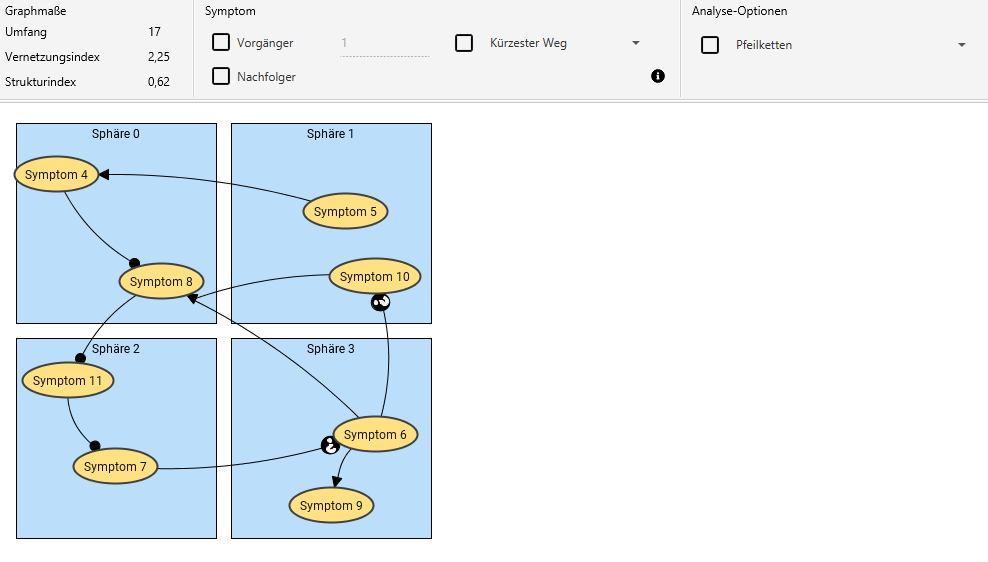
\includegraphics[width=1\columnwidth, keepaspectratio]{analyse.png} 
	}
	\caption{Analyse Optionen}
\end{figure}

\begin{figure}[ht!]
	\centering
	\subfigure{
		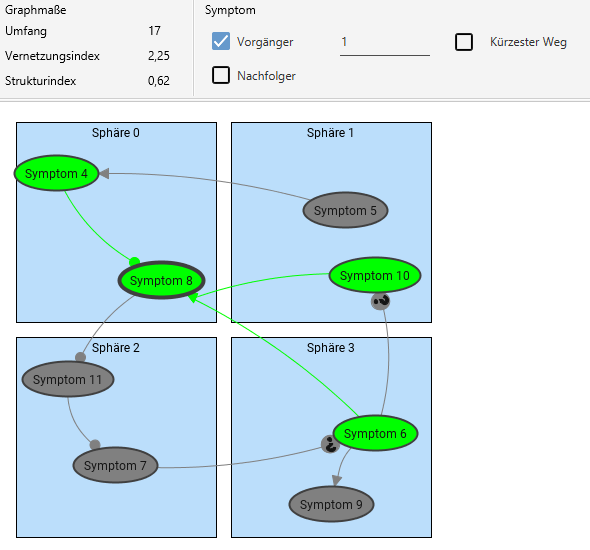
\includegraphics[width=0.6\columnwidth, keepaspectratio]{analyse2.png} 
	}
	\caption{Analyse Optionen (2)}
\end{figure}


%%%%%%%%%%%%%%%%%%%%%%%%%%%%%%%%%%%%%%%%%%%%%%%%%%%%%%%%%%%%%%%%%%%%%%%%%%%%%%%%%%%%%%%%%%%%%%%%%%%%%%%%%%%%%%%%%%%
\newpage
\subsubsection{Graphmaße} 
	\condition 
	Das Programm ist geöffnet und ein Syndrom wird angezeigt.
	\action
	\begin{enumerate}
		\item Graphmaße (Umfang, Vernetzungsindex und Strukturindex) werden in der Leiste oben links angezeigt und können dort abgelesen werden.
	\end{enumerate} 
	\hint
	\begin{itemize}
		\item Diese Maße beziehen sich auf das gesamte Syndrom. Es ist dabei unabhängig, welche Graphelemente aktuell ausgewählt sind.
		\item Die Graphmaße werden automatisch beim Öffnen des Analysemodus berechnet. \\
	\end{itemize}

\newpage
%%%%%%%%%%%%%%%%%%%%%%%%%%%%%%%%%%%%%%%%%%%%%%%%%%%%%%%%%%%%%%%%%%%%%%%%%%%%%%%%%%%%%%%%%%%%%%%%%%%%%%%%%%%%%%%%%%%
\subsubsection{Vorgänger/ Nachfolger von Symptom(en) hervorheben}
	\condition 
		Das Programm ist geöffnet und ein Syndrom wird angezeigt.
	\action
	\begin{enumerate}
		\item Das Symptom, zu dem die Vorgänger und/oder Nachfolger angezeigt werden sollen, mit einem Links-Klick auswählen.
		\item Die entsprechenden Checkboxen Vorgänger und/ oder Nachfolger aktivieren und die Anzahl wie viele Vorgänger / Nachfolger im Graphen angezeigt werden soll. Die Eingabe mit der \textit{Enter}-Taste bestätigen.
		\item Durch einen erneuten Links-Klick in eine Checkbox kann diese wieder abgewählt werden. Durch Eingabe einer anderen Zahl in dem Feld neben den Boxen und anschließender Bestätigung der Eingabe mit der \textit{Enter}-Taste kann die Anzahl an Vorgängern / Nachfolgern angepasst werden.
	\end{enumerate} 
	\hint
	\begin{itemize}
		\item Die Vorgänger und Nachfolger sowie das ausgewählte Symptom/ die ausgewählten Symptome werden farblich hervorgehoben dargestellt, während die übrigen Symptome grau visualisiert werden. \\
	\end{itemize}

%%%%%%%%%%%%%%%%%%%%%%%%%%%%%%%%%%%%%%%%%%%%%%%%%%%%%%%%%%%%%%%%%%%%%%%%%%%%%%%%%%%%%%%%%%%%%%%%%%%%%%%%%%%%%%%%%%%
\subsubsection{Kürzester Pfad zw. Symptomen}
	\condition 
		Das Programm ist geöffnet und ein Syndrom mit mindestens zwei Symptomen, die durch eine Relation verbunden sind, ist geöffnet.
	\action
	\begin{enumerate}
		\item Das Symptom, welches als Startknoten gelten soll, mit einem Links-Klick auswählen.
		\item Die \textit{Shift}-Taste der Tastatur drücken und gedrückt halten.
		\textit Das Symptom, welches als Zielknoten gelten soll, mit einem Links-Klick auswählen.
		\item Die \textit{Shift}-Taste loslassen.
		\item In der oberen Leiste im Bereich Symptome auf den Button \textit{Die Wege zwischen zwei Symptomen anzeigen} einen Links-Klick ausführen.
		\item In dem sich öffnenden Drop-Down-Menü die Option \textit{Kürzester Weg} durch einem Links-Klick auswählen.
		\item In der oberen Leiste im Bereich Symptome einen Links-Klick in die Checkbox links neben dem Button \textit{Die Wege zwischen zwei Symptomen anzeigen} ausführen, sodass ein Haken in diesem Feld gesetzt ist.
	\end{enumerate} 
	\hint
	\begin{itemize}
		\item Die Reihenfolge, in der die Symptome ausgewählt werden, ist wichtig, da die Relationen gerichtet verlaufen. 
		\item Der Startknoten, der Zielknoten sowie alle Symptome, die auf dem kürzesten Weg zwischen dem Start- und dem Ziel-Symptom liegen werden farblich hervorgehoben ebenso die Relationen, die den kürzesten Weg bilden. Die übrigen Symptome und Relationen werden dagegen grau visualisiert. \\
	\end{itemize}

%%%%%%%%%%%%%%%%%%%%%%%%%%%%%%%%%%%%%%%%%%%%%%%%%%%%%%%%%%%%%%%%%%%%%%%%%%%%%%%%%%%%%%%%%%%%%%%%%%%%%%%%%%%%%%%%%%%
\subsubsection{Alle Pfade zw. Symptomen}
	\condition 
		Das Programm ist geöffnet und ein Syndrom mit mindestens zwei Symptomen, die durch eine Relation verbunden sind, ist geöffnet.
	\action
	\begin{enumerate}
		\item Das Symptom, welches als Startknoten gelten soll, mit einem Links-Klick auswählen.
		\item Die \textit{Shift}-Taste der Tastatur drücken und gedrückt halten.
		\textit Das Symptom, welches als Zielknoten gelten soll, mit einem Links-Klick auswählen.
		\item Die \textit{Shift}-Taste loslassen.
		\item In der oberen Leiste im Bereich Symptome auf den Button \textit{Die Wege zwischen zwei Symptomen anzeigen} einen Links-Klick ausführen.
		\item In dem sich öffnenden Drop-Down-Menü die Option \textit{Alle Wege} durch einem Links-Klick auswählen.
		\item In der oberen Leiste im Bereich Symptome einen Links-Klick in die Checkbox links neben dem Button \textit{Die Wege zwischen zwei Symptomen anzeigen} ausführen, sodass ein Haken in diesem Feld gesetzt ist.
	\end{enumerate} 
	\hint
	\begin{itemize}
		\item Die Reihenfolge, in der die Symptome ausgewählt werden, ist wichtig, da die Relationen gerichtet verlaufen. 
		\item Der Startknoten, der Zielknoten sowie alle Symptome, die auf einem Weg zwischen dem Start- und dem Ziel-Symptom liegen werden farblich hervorgehoben, ebenso die Relationen, die diese Wege bilden. Die übrigen Symptome und Relationen werden dagegen grau visualisiert.\\
	\end{itemize}

%%%%%%%%%%%%%%%%%%%%%%%%%%%%%%%%%%%%%%%%%%%%%%%%%%%%%%%%%%%%%%%%%%%%%%%%%%%%%%%%%%%%%%%%%%%%%%%%%%%%%%%%%%%%%%%%%%%
\subsubsection{Pfeilketten}
	\condition 
		Das Programm ist geöffnet und ein Syndrom wird angezeigt.
	\action
	\begin{enumerate}
		\item In der oberen Leiste im Bereich Analyse-Optionen die Checkbox \textit{Analyse-Optionen aktivieren} durch einen Links-Klick aktivieren, sodass ein Haken gesetzt ist und auf die Liste daneben drücken.
		\item In dem sich öffnenden Drop-Down-Menü die Option \textit{Pfeilketten} mit einem Links-Klick auswählen. 
		\item Durch einen erneuten Links-Klick in die Checkbox kann die Auswahl der Option deaktiviert werden.
	\end{enumerate} 
	\hint
	\begin{itemize}
		\item Der Symptome und Relationen, die Teil eines Zyklus sind, werden farblich hervorgehoben. Die übrigen Symptome und Relationen werden dagegen grau visualisiert.\\
	\end{itemize}

%%%%%%%%%%%%%%%%%%%%%%%%%%%%%%%%%%%%%%%%%%%%%%%%%%%%%%%%%%%%%%%%%%%%%%%%%%%%%%%%%%%%%%%%%%%%%%%%%%%%%%%%%%%%%%%%%%%
\subsubsection{Konvergente Verzweigungen}
	\condition 
	Das Programm ist geöffnet und ein Syndrom wird angezeigt.
	\action
	\begin{enumerate}
		\item In der oberen Leiste im Bereich Analyse-Optionen in as Feld \textit{Analyse-Optionen aktivieren} einen Links-Klick ausführen.
		\item In dem sich öffnenden Drop-Down-Menü die Option \textit{Konvergente Verzweigungen} mit einem Links-Klick auswählen. 
		\item Sofern noch kein Haken in der Checkbox links neben diesem Feld ist, einen Links-Klick in diese Box ausführen, sodass ein Haken gesetzt ist.
		\item Durch einen erneuten Links-Klick in dieses Feld kann die Auswahl der Option deaktiviert werden.
	\end{enumerate} 
	\hint
	\begin{itemize}
		\item Der Symptome und Relationen, die konvergente Verzweigungen darstellen, werden farblich hervorgehoben. Die übrigen Symptome und Relationen werden dagegen grau visualisiert. \\
	\end{itemize}

%%%%%%%%%%%%%%%%%%%%%%%%%%%%%%%%%%%%%%%%%%%%%%%%%%%%%%%%%%%%%%%%%%%%%%%%%%%%%%%%%%%%%%%%%%%%%%%%%%%%%%%%%%%%%%%%%%%
\subsubsection{Divergente Verzweigungen}
	\condition 
	Das Programm ist geöffnet und ein Syndrom wird angezeigt.
	\action
	\begin{enumerate}
		\item In der oberen Leiste im Bereich Analyse-Optionen in as Feld \textit{Analyse-Optionen aktivieren} einen Links-Klick ausführen.
		\item In dem sich öffnenden Drop-Down-Menü die Option \textit{Divergente Verzweigungen} mit einem Links-Klick auswählen. 
		\item Sofern noch kein Haken in der Box links neben diesem Feld ist, einen Links-Klick in diese Box ausführen, sodass ein Haken erscheint.
		\item Durch einen erneuten Links-Klick in dieses Feld kann die Auswahl der Option deaktiviert werden.
	\end{enumerate} 
	\hint
	\begin{itemize}
		\item Der Symptome und Relationen, die divergente Verzweigungen darstellen, werden farblich hervorgehoben. Die übrigen Symptome und Relationen werden dagegen grau visualisiert. \\
	\end{itemize}
\newpage
%%%%%%%%%%%%%%%%%%%%%%%%%%%%%%%%%%%%%%%%%%%%%%%%%%%%%%%%%%%%%%%%%%%%%%%%%%%%%%%%%%%%%%%%%%%%%%%%%%%%%%%%%%%%%%%%%%%
\subsubsection{Alle Verzweigungen}
	\condition 
	Das Programm ist geöffnet und ein Syndrom wird angezeigt.
	\action
	\begin{enumerate}
		\item In der oberen Leiste im Bereich Analyse-Optionen in as Feld \textit{Analyse-Optionen aktivieren} einen Links-Klick ausführen.
		\item In dem sich öffnenden Drop-Down-Menü die Option \textit{Verzweigungen} mit einem Links-Klick auswählen. 
		\item Sofern noch kein Haken in der Box links neben diesem Feld ist, einen Links-Klick in diese Box ausführen, sodass ein Haken erscheint.
		\item Durch einen erneuten Links-Klick in dieses Feld kann die Auswahl der Option deaktiviert werden.
	\end{enumerate} 
	\hint
	\begin{itemize}
		\item Der Symptome und Relationen, die konvergente oder divergente Verzweigungen darstellen, werden farblich hervorgehoben. Die übrigen Symptome und Relationen werden dagegen grau visualisiert. \\
	\end{itemize}

%%%%%%%%%%%%%%%%%%%%%%%%%%%%%%%%%%%%%%%%%%%%%%%%%%%%%%%%%%%%%%%%%%%%%%%%%%%%%%%%%%%%%%%%%%%%%%%%%%%%%%%%%%%%%%%%%%%
\subsubsection{Zyklen}
	\condition 
	Das Programm ist geöffnet und ein Syndrom wird angezeigt.
	\action
	\begin{enumerate}
		\item In der oberen Leiste im Bereich Analyse-Optionen in as Feld \textit{Analyse-Optionen aktivieren} einen Links-Klick ausführen.
		\item In dem sich öffnenden Drop-Down-Menü die Option \textit{Zyklen} mit einem Links-Klick auswählen. 
		\item Sofern noch kein Haken in der Box links neben diesem Feld ist, einen Links-Klick in diese Box ausführen, sodass ein Haken erscheint.
		\item Durch einen erneuten Links-Klick in dieses Feld kann die Auswahl der Option deaktiviert werden.
	\end{enumerate} 
	\hint
	\begin{itemize}
		\item Der Symptome und Relationen, die Zyklen darstellen, werden  farblich hervorgehoben. Die übrigen Symptome und Relationen werden dagegen grau visualisiert. \\
	\end{itemize}
	
\newpage	
%%%%%%%%%%%%%%%%%%%%%%%%%%%%%%%%%%%%%%%%%%%%%%%%%%%%%%%%%%%%%%%%%%%%%%%%%%%%%%%%%%%%%%%%%%%%%%%%%%%%%%%%%%%%%%%%%%%
\subsection{Verlauf der Nutzerinteraktionen} \label{logs}
Dieser Abschnitt beschäftigt sich mit dem Protokoll der Nutzerinteraktionen. Dieses kann als ganzes angezeigt werden, sodass die Graph-Erstellung und Bearbeitung in ihrer chronologischen Reihenfolge nachvollzogen werden kann. Die Nutzerinteraktionen können allerdings auch nach verschiedenen Aktionen gefiltert werden. Diese Funktionalität stellt nur der Analysemodus zur Verfügung. Deswegen wird im Folgenden davon ausgegangen, dass der Benutzer diesen in der Anwendung geöffnet hat.  \\
%%%%%%%%%%%%%%%%%%%%%%%%%%%%%%%%%%%%%%%%%%%%%%%%%%%%%%%%%%%%%%%%%%%%%%%%%%%%%%%%%%%%%%%%%%%%%%%%%%%%%%%%%%%%%
\subsubsection{Anzeigen}
	\condition 
		Das Programm ist geöffnet.
	\action
	\begin{enumerate}
		\item Einen Links- Klick auf \textit{Verlauf} (unter der Übersichtsleiste) ausführen, sodass sich die dazugehörige Leiste ausklappt.
		\item Einen Links-Klick auf das Synchronisations- Symbol ausführen.
		\item Die Nutzerinteraktionen können in dieser Leiste gelesen werden. 
		\item Durch einen erneuten Links-Klick auf \textit{Verlauf} klappt sich die Leiste wieder ein.
	\end{enumerate} 
	\hint
	\begin{itemize}
		\item Die Liste von Nutzeraktionen wird in der Leiste angezeigt. Dabei steht die zuerst durchgeführte Aktion ganz oben und die zuletzt durchgeführte Aktion ganz unten in der Liste.
		\item Die Stellen in der Liste, an denen sich Pfeile befinden können mit einem Links-Klick ein-/ ausgeklappt werden, um die Übersichtlichkeit zu erhöhen oder erweiternde Informationen angezeigt zu bekommen. 
	\end{itemize}

%%%%%%%%%%%%%%%%%%%%%%%%%%%%%%%%%%%%%%%%%%%%%%%%%%%%%%%%%%%%%%%%%%%%%%%%%%%%%%%%%%%%%%%%%%%%%%%%%%%%%%%%%%%%%
\subsubsection{Filtern}
	\condition 
	Das Programm ist geöffnet.
	\action
	\begin{enumerate}
		\item Einen Links- Klick auf \textit{Verlauf} (unter der Übersichtsleiste) ausführen, sodass sich die dazugehörige Leiste ausklappt.
		\item Einen Links- Klick auf das Synchronisations- Symbol ausführen.
		\item Einen Links- Klick auf das Feld neben dem Synchronisations- Symbol ausführen.
		\item In dem sich öffnenden Drop-Down-Menü die Option wählen, nach der die Liste aller Nutzerinteraktionen gefiltert werden soll.
		\item Die gefilterten Nutzerinteraktionen können nun gelesen werden. 
		\item Durch einen erneuten Links-Klick auf \textit{Verlauf} klappt sich die Leiste wieder ein.
	\end{enumerate} 
	\hint 
	\begin{itemize}
		\item Die (gefilterte) Liste von Nutzeraktionen wird in der Leiste angezeigt. Dabei steht die zuerst durchgeführte Aktion ganz oben und die zuletzt durchgeführte Aktion ganz unten in der Liste.
		\item Die Stellen in der Liste, an denen sich Pfeile befinden können mit einem Links-Klick eingeklappt werden, um die Übersichtlichkeit zu erhöhen, oder ausgeklappt werden, wenn zusätzliche Informationen angezeigt werden sollen.
	\end{itemize}

	\begin{figure}[ht!]
		\centering
		\subfigure{
			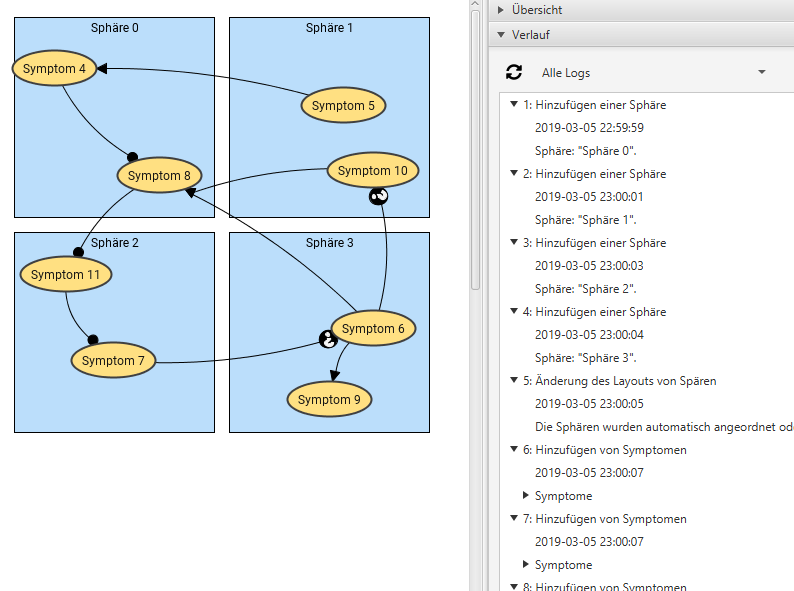
\includegraphics[width=0.7\columnwidth, keepaspectratio]{logs.png} 
		}
		\caption{Verlauf(1)}
	
	\end{figure}

	\begin{figure}[ht!]
		\centering
		\subfigure{
			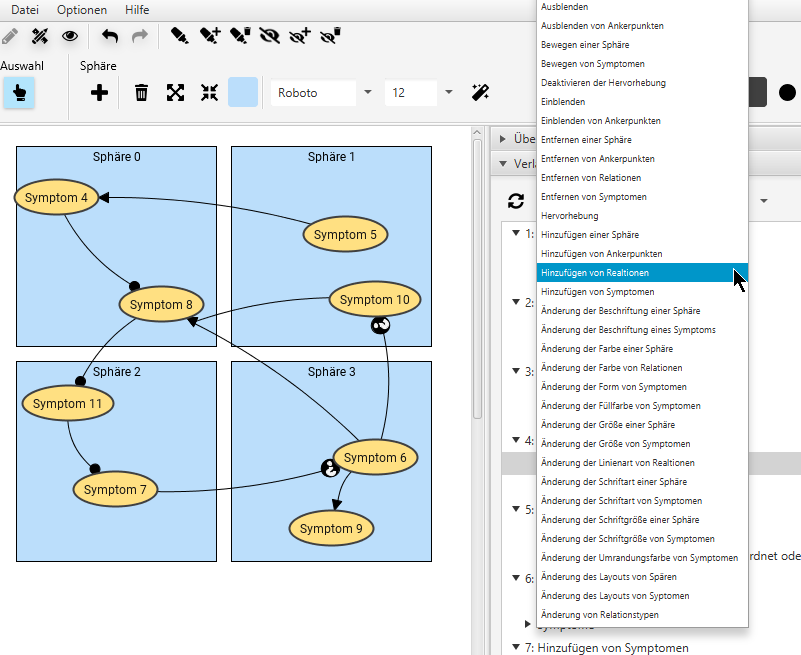
\includegraphics[width=0.7\columnwidth, keepaspectratio]{logs2.png} 
		}
		\caption{Verlauf(2)}
	
	\end{figure}
%%%%%%%%%%%%%%%%%%%%%%%%%%%%%%%%%%%%%%%%%%%%%%%%%%%%%%%%%%%%%%%%%%%%%%%%%%%%%%%%%%%%%%%%%%%%%%%%%%%%%%%%%%%%%		
		

\clearpage
%%%%%%%%%%%%%%%%%%%%%%%%%%%%%%%%%%%%%%%%%%%%%%%%%%%%%%%%%%%%%%%%%%%%%%%%%%%%%%%%%%%%%%%%%%%%%%%%%%%%%%%%%%%%%%%%%%%%
\subsection{Vorlage} \label{template}
Eine Vorlage kann als ein spezielles Syndrom angesehen werden. Neben dem eigentlichen Syndrom (also einer Menge an Sphären, Knoten und Kanten) enthält eine Vorlage zusätzliche Informationen. Diese Informationen legen fest, in wie weit ein das enthaltene Syndrom bearbeitet werden kann. Dies beinhaltet sowohl Regeln, wie viele Sphären, Symptome und Kanten hinzugefügt werden können, als auch Festlegungen zu jedem einzelnen aktuell im Syndrom enthaltenen Graphelement. Letztere Regelungen, die die einzelnen schon vorhandenen Graphelemente betreffen unterscheiden sich. Die Regeln für Sphären unterscheiden sich von den Regeln der Symptome und diese sind wiederum anders als die Regeln von Relationen. \\ \\
Es können folgende Regeln eingestellt werden, die sich anschließend auf die Bearbeitung des Syndroms auswirken: \\ \\
\textbf{\bbe{Regeln für das gesamte Syndrom:}}
\begin{enumerate}
	\item die maximale Anzahl an Sphären im Syndrom
	\item die maximale Anzahl an Symptomen im Syndrom 
	\item die maximale Anzahl an Relationen im Syndrom
	\item die im Syndrom erlaubten Relationstypen
\end{enumerate}

\textbf{\bbe{Regeln für einzelne Sphären}}\\
(folgende Eigenschaften der gewählten Sphäre können gesperrt werden, sodass diese nicht mehr verändert werden können): 
\begin{enumerate}
	\item der Titel der Sphäre (beinhaltet den Titel sowie dessen Schriftart und -größe)
	\item die Position der Sphäre
	\item der Style der Sphäre (beinhaltet die Größe und Füllfarbe)
	\item die Möglichkeit, die in dieser Sphäre enthaltenen Symptome zu löschen und in diese Sphäre weitere Symptome hinzuzufügen
	\item Festlegung der maximal in dieser Sphäre enthaltenen Symptome
	\item Hinweis: Ist einer dieser Werte gesperrt, so kann die Sphäre nicht gelöscht werden.
\end{enumerate}
\textbf{\bbe{Regeln für einzelne Symptome}}\\
(folgende Eigenschaften des gewählten Symptoms können gesperrt werden, sodass diese nicht mehr verändert werden können):
\begin{enumerate}
	\item der Titel des Symptoms (beinhaltet den Titel sowie dessen Schriftart und -größe)
	\item die Position des Symptoms
	\item der Style das Symptoms (beinhaltet die Größe, Füllfarbe und Randfarbe)
	\item Hinweis: Ist einer dieser Werte gesperrt, so kann das Symptom nicht gelöscht werden.
\end{enumerate}
\textbf{\bbe{Regeln für einzelne Relationen}}\\
(folgende Eigenschaften der gewählten Relation können gesperrt werden, sodass diese nicht mehr verändert werden können):
\begin{enumerate}
	\item die Position der Relation (betrifft in erster Linie das Setzen oder Verändern von Ankerpunkten)
	\item der Style der Relation (betrifft die Farbe sowie die Kantenart)
	\item der Relationstyp
	\item Hinweis: Ist einer dieser Werte gesperrt, so kann die Relation nicht gelöscht werden.
\end{enumerate}

Durch Festlegung der einzelnen Werte kann die Bearbeitung und Erweiterung des Graphen festgelegt werden.

	\begin{figure}[ht!]
		\centering
		\subfigure{
			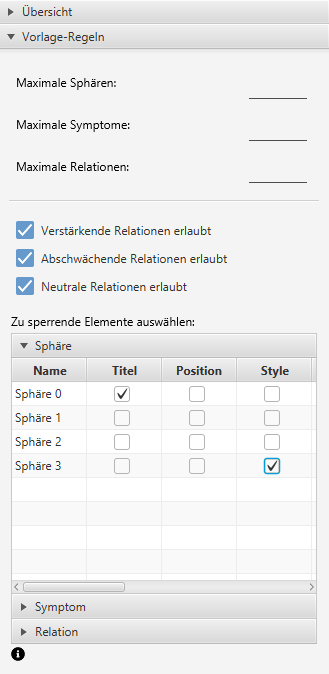
\includegraphics[width=0.4\columnwidth, keepaspectratio]{template.png} 
		}
		\caption{Vorlage}
		
	\end{figure}


%%%%%%%%%%%%%%%%%%%%%%%%%%%%%%%%%%%%%%%%%%%%%%%%%%%%%%%%%%%%%%%%%%%%%%%%%%%%%%%%%%%%%%%%%%%%%%%%%%%%%%%%%%%%%%%%%%%%
\subsubsection{Vorlage erstellen}
Zur Erstellung einer Vorlage muss der Ersteller-Modus der Anwendung aktiv sein. Nur in diesem Modus ist es möglich Regeln für die spätere Bearbeitung des Syndroms festzulegen. Die einmal eingestellten Regeln können dabei jederzeit bedarfsgerecht angepasst werden. Hierzu können eingegebene Werte verändert und ausgewählte Optionen wieder deselektiert (und damit aus der Auswahl entfernt) werden. In den folgenden beiden Unterkapiteln werden die Aktionen beschrieben, die für die Erstellung einer Vorlage relevant sind. \\
%%%%%%%%%%%%%%%%%%%%%%%%%%%%%%%%%%%%%%%%%%%%%%%%%%%%%%%%%%%%%%%%%%%%%%%%%%%%%%%%%%%%%%%%%%%%%%%%%%%%%%%%%%%%%%%%%%%%
\newpage
\subsubsection{Graph spezifische Vorlageregeln}
	\condition 
		Das Programm ist geöffnet und der Ersteller-Modus ist aktiv.
	\action
	\begin{enumerate}
		\item Einen Linksklick auf \textit{Vorlage-Regeln} (unter der Übersichtsleiste) ausführen, sodass sich die dazugehörige Leiste ausklappt.
		\item Im oberen Bereich dieser Leiste kann in den Feldern neben den Beschriftungen \textit{Maximal Sphären}, \textit{Maximal Symptome} und \textit{Maximal Relationen} jeweils die maximale Anzahl eingegeben werden, die es von diesem Graphelement-Typ im Syndrom geben darf. Hierzu mit einem Links-Klick in das gewünschte Feld klicken und anschließend über die Tastatur die gewünschte Zahl (als Ziffer/ Ziffernfolge) eingegeben werden. Mit der \textit{Enter}-Taste wird die Eingabe bestätigt werden.
		\item Unter diesen drei Eingabefelder findet sich ein Bereich in dem die Relationstypen, die bei der Bearbeitung des Syndroms erlaubt sind, eingestellt werden können. Standardmäßig sind alle Relationstypen erlaubt. Um einen Relationstyp für die Bearbeitung zu sperren einen Links-Klick in die Box neben dem entsprechenden Relationstyp ausführen, sodass der Haken in dieser Box verschwindet. Durch einen erneuten Links-Klick in die entsprechende Checkbox wird wieder ein Haken gesetzt und der entsprechende Relationstyp kann wieder in der Bearbeitung verwendet werden.
	\end{enumerate} 
	\hint
	\begin{itemize}
		\item Es können keine negativen Zahlen und auch kein Text in die Felder für die maximale Anzahl eines Graphelement-Typs eingegeben werden. \\
	\end{itemize}
%%%%%%%%%%%%%%%%%%%%%%%%%%%%%%%%%%%%%%%%%%%%%%%%%%%%%%%%%%%%%%%%%%%%%%%%%%%%%%%%%%%%%%%%%%%%%%%%%%%%%%%%%%%%%%%%%%%%
\subsubsection{Element spezifische Vorlageregeln}
	\condition 
	Das Programm ist geöffnet und der Ersteller-Modus ist aktiv.
	\action
	\begin{enumerate}
		\item Einen Linksklick auf \textit{Vorlage-Regeln} (unter der Übersichtsleiste) ausführen, sodass sich die dazugehörige Leiste ausklappt.
		\item Im unteren Bereich dieser Leiste sind unter dem Text \textit{Zu sperrende Elemente auswählen:} die drei Spalten \textit{Sphäre}, \textit{Symptom} und \textit{Relation} zu finden. Durch einen Links-Klick auf eine dieser Spalten kann die dazugehörige Leiste ausgeklappt werden. In dieser Leiste stehen jeweils die Elemente des Syndrom dieses Graphelement-Typs untereinander aufgelistet. Um die Eigenschaften eines dieser Elemente zu sperren einen Links-Klick in das Feld der Eigenschaft, die für das Element gesperrt werden soll, dessen Titel am Anfang der Zeile steht. Es erscheint ein Haken in der Box und die Eigenschaft dieses Elements wurde gesperrt. Durch einen erneuten Links-Klick in die Box kann die Sperrung der Eigenschaft aufgehoben werden.
	\end{enumerate} 
	\hint
	\begin{itemize}
		\item Es kann für verschiedene Elemente eine unabhängige Kombination an gesperrten Elementen vorgenommen werden. \\
	\end{itemize} 

%%%%%%%%%%%%%%%%%%%%%%%%%%%%%%%%%%%%%%%%%%%%%%%%%%%%%%%%%%%%%%%%%%%%%%%%%%%%%%%%%%%%%%%%%%%%%%%%%%%%%%%%%%%%%%%%%%%%
\subsubsection{Vorlage verwenden}
Damit die in der Vorlage hinterlegten Regeln sich auf die Bearbeitung des Syndroms auswirken, muss der Bearbeiter-Modus der Anwendung aktiv sein.\\
Dabei ist bei der Verwendung einer Vorlage zu beachten, dass Aktionen (wie beispielsweise das Ändern der Farbe eines Graphelements), die vom Programm grundsätzlich zur Verfügung gestellt werden, unter Umständen nicht mehr zu funktionieren scheinen. Dieser Eindruck kann dadurch entstehen, dass der Aufruf bestimmter Aktionen zu keiner Änderung des angezeigten Syndroms führt. Hinweise in der Benutzeroberfläche sollen diesen Fehleindruck eines unerwünschten Programmverhaltens verhindern. \\
Die angezeigten Hinweise geben Aufschluss darüber, dass die Aktion deshalb nicht umgesetzt werden kann, weil die angeforderte Aktion durch die Regeln in der Vorlage untersagt wird. \\

%%%%%%%%%%%%%%%%%%%%%%%%%%%%%%%%%%%%%%%%%%%%%%%%%%%%%%%%%%%%%%%%%%%%%%%%%%%%%%%%%%%%%%%%%%%%%%%%%%%%%%%%%%%%%%%%%%%%
\subsection{Benutzermodus wechseln}
	\condition 
		Das Programm ist geöffnet.
	\action
	\begin{enumerate}
		\item In der Menüleiste befinden sich oben links die drei Buttons \textit{Bearbeiter-Modus}, \textit{Ersteller-Modus} und \textit{Analyse-Modus}. Der gewünschte Modus kann durch einen Links-Klick auf den entsprechenden Button ausgewählt werden.
	\end{enumerate} 
	\hint
	\begin{itemize}
		\item Es kann immer nur ein Modus zur Zeit aktiv sein. Die Modi können also nicht zeitgleich kombiniert werden.
		\item Während der Benutzung der Anwendung kann beliebig zwischen den Funktionsmodi gewechselt werden. \\
\end{itemize}			 
		
\newpage
%%%%%%%%%%%%%%%%%%%%%%%%%%%%%%%%%%%%%%%%%%%%%%%%%%%%%%%%%%%%%%%%%%%%%%%%%%%%%%%%%%%%%%%%%%%%%%%%%%%%%%%%%%%%%		
\subsection{Dialogfenster} \label{dialog}
\subsubsection{Informationsdialog}
Während der Nutzung des Programms kann es dazu kommen, dass sich ein Fenster öffnet, dass erst bestätigt werden muss, bevor weitere Aktionen ausgeführt werden können. \\
Diese Dialogfenster geben wichtige Hinweise für das Ergebnis der aktuellen (also zuletzt aufgerufenen Aktion). \bbe{Sie sollten also unbedingt gelesen werden.} \\
Die Info Dialoge bieten 2 Möglichkeiten das Dialogfenster zu schließen. Einen \textit{Weiter}- und einen \textit{Abbrechen}- Button. Wie die Bezeichnungen der Buttons suggerieren, wird bei Klick auf \textit{Weiter} die gewählte Aktion fortgeführt, während der Klick auf \textit{Abbrechen} die Aktion abbricht. \\
Ein Info Dialog wird beispielsweise geöffnet, wenn ein neues Syndrom erstellt oder importiert werden soll. \\

\textbf{Beispiel:}
	\begin{enumerate}
		\item In der obersten Menüleiste \texttt{Datei/ Neue Datei} auswählen. Somit soll ein neues Syndrom erstellt werden.
		\item Der Informationsdialog öffnet sich.
		\item Durch einen Links-Klick auf \textit{Weiter} wird ein neues Syndrom erstellt. Das Syndrom welches zuvor in \textbf{GraphIt} geladen war, wird überschrieben. 
		\item Durch einen Links-Klick auf \textit{Abbrechen} wird kein neuer Graph erstellt, sodass der aktuell in der GUI angezeigte Graph weiter bearbeitet werden kann. 
	\end{enumerate}
Ähnlich verhält es sich bei den anderen Dialogfenstern der Anwendung.\\
	\begin{figure}[ht!]
	\centering
	\subfigure{
		
\includegraphics[width=0.8\columnwidth, keepaspectratio]{info_dialog.png} 
	}
	\caption{Informationsdialog}
\end{figure}

\newpage
%%%%%%%%%%%%%%%%%%%%%%%%%%%%%%%%%%%%%%%%%%%%%%%%%%%%%%%%%%%%%%%%%%%%%%%%%%%%%%%%%%%%%%%%%%%%%%%%%%%%%%%%%%%%%%%%%
	
\subsubsection{File Chooser} 
Bei einem File Chooser (Dateiauswahl) handelt es sich um das Fenster, dass die Auswahl eines Dateipfades ermöglicht. Dieses Fenster öffnet sich also stets, wenn es darum geht eine Datei zu speichern/ exportieren/ öffnen oder zu importieren. 

\textbf{Exportieren/ Speichern}
\action
\begin{enumerate}
	\item In das Textfeld \textit{Dateiname} den gewünschten Namen der Datei eintragen. 
	\item Über das Hauptfenster an den gewünschten Speicherort navigieren. 
	\item Zum erfolgreichen Abschließen der Aktion auf den \textit{Speichern}- Button klicken. Zum Abbrechen auf den \textit{Abbrechen}- Button auswählen.
\end{enumerate}

\textbf{Öffnen/ Importieren}
\action
\begin{enumerate}
	\item Über das Textfeld \textit{Dateiname} können Dateien in dem derzeitigen Ordner gesucht werden.
	\item Über das Hauptfenster an den gewünschten Speicherort navigieren und die zu öffnende/ importierende Datei auswählen.
	\item Zum erfolgreichen Abschließen der Aktion auf den \textit{Öffnen}- Button klicken. Zum Abbrechen auf den \textit{Abbrechen}- Button auswählen.
\end{enumerate}

 \begin{figure}[ht!]
 	\centering
 	\subfigure[Exportieren/ Speichern]{
 		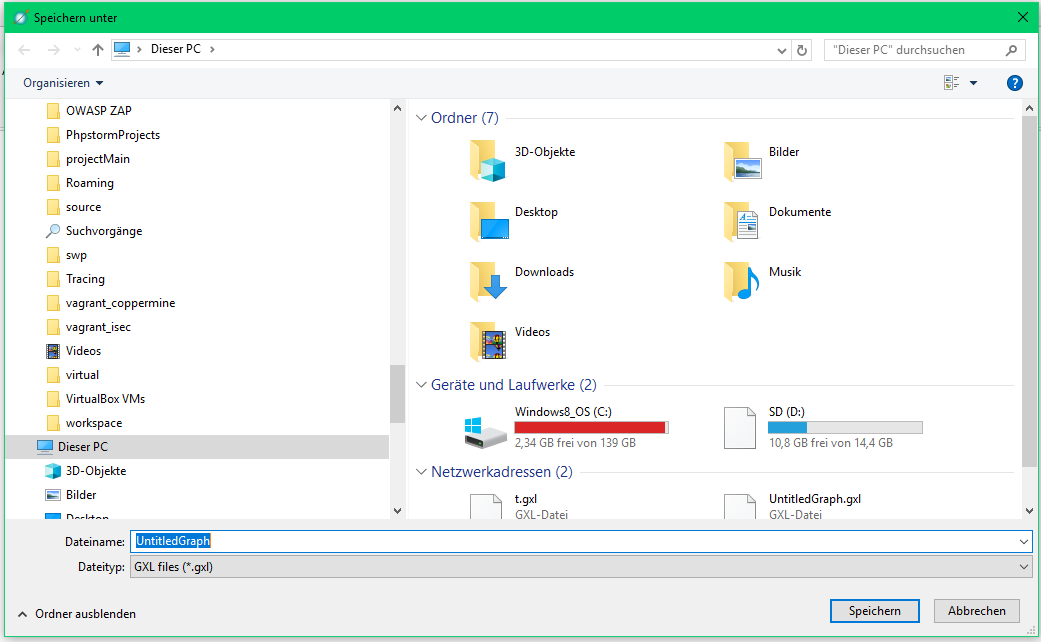
\includegraphics[width=0.45\columnwidth, keepaspectratio]{save.png} 
 	}
 	\subfigure[Öffnen/ Importieren]{
 		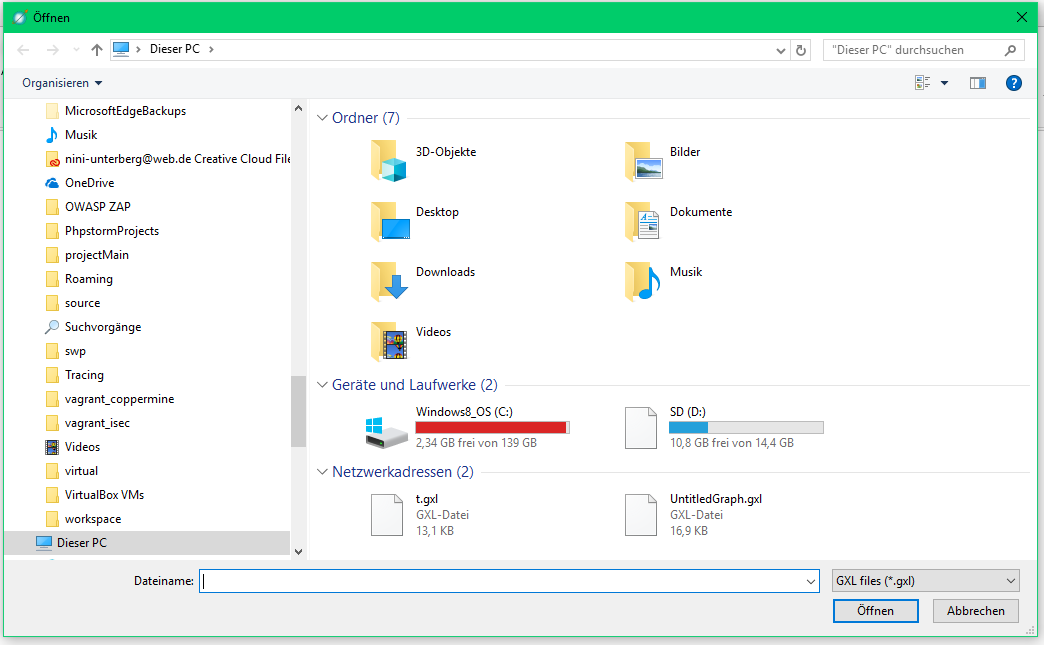
\includegraphics[width=0.45\columnwidth, keepaspectratio]{open.png} 
 	}
 	\caption{File Chooser}	
 \end{figure}

\newpage
%%%%%%%%%%%%%%%%%%%%%%%%%%%%%%%%%%%%%%%%%%%%%%%%%%%%%%%%%%%%%%%%%%%%%%%%%%%%%%%%%%%%%%%%%%%%%%%%%%
\subsection{Druckdialog}
Beim Druckdialog handelt es sich um ein Dialog-Fenster, das der Anpassung der Druck-Einstellungen ermöglicht. So können Einstellungen nach benutzerspezifischen Präferenzen vorgenommen werden. Mögliche Einstellungen sind zum Beispiel die Anzahl an zu erstellenden Exemplaren und das für den Druckauftrag zu verwendende Drucker-Gerät.
Auch dieses Dialogfenster bietet zwei mögliche Ergebnisse, mit denen das Fenster geschlossen werden kann.
\begin{itemize}
	\item Durch einen Links-Klick auf \textit{OK} wird der Druckauftrag an den Drucker geleitet. Das in der Benutzeroberfläche angezeigte Syndrom (beziehungsweise der dort zu sehende Ausschnitt des Syndroms) wird am eingestellten Drucker in der angeforderten Anzahl gedruckt. 
	\item Ein Links-Klick auf \textit{Abbrechen} sorgt dafür, dass kein Druck angefertigt wird.
\end{itemize}

\hint
\begin{itemize}
	\item Es wird nur der Bereich des Syndroms gedruckt, der gerade auch im Hauptfenster sichtbar ist.
	\item Die Druckeinstellungen erscheinen womöglich im Hintergrund, d.h. durch Bewegen der Maus auf das Icon von \textbf{GraphIt} in der Symbolleiste, kann durch Auswählen des dort erscheinenden Druckfensters dieses in den Vordergrund geholt werden. 
\end{itemize}

%%%%%%%%%%%%%%%%%%%%%%%%%%%%%%%%%%%%%%%%%%%%%%%%%%%%%%%%%%%%
\subsubsection{Color Picker} \label{colorpicker}
Ein Color Picker (\textit{Farbwähler}) dient der Auswahl einer Farbe. 
\action
\begin{enumerate}
	\item Einen der entsprechende Farb- Buttons (\textit{Hintergrundfarbe der Sphäre verändern}, \textit{Hintergrundfarbe des Symptoms verändern}, \textit{Randfarbe des Symptoms verändern}, \textit{Farbe de Relation verändern}) durch einen Links- oder Rechts-Klick auswählen. 
	\item Aus dem sich öffnenden  Drop-Down-Menü eine Farbe per Links- Klick auswählen. 
\end{enumerate}
\hint
\begin{itemize}
	\item Die Aktion kann durch einen Klick außerhalb des Color Pickers oder durch einen Rechts- Klick innerhalb des Color Pickers abgebrochen werden. 
\end{itemize}

\textbf{Custom Color}\\
Falls die gewünschte Farbe nicht in dem Drop-Down-Farbmenü des Color Pickers enthalten ist, kann eine benutzerdefinierte Farbe/ Custom Color ausgewählt werden. 
\action
\begin{enumerate}
	\item Dazu wie in der vorgehenden Anleitung den Color Picker öffnen. Am unten Rand des Color Pickers auf den Schriftzug \textit{Custom Color} klicken. 
	\item Auf dem sich öffnenden Dialog kann nun eine Farbe ausgewählt werden. 
	\item In den beiden äußeren Farbringen kann der Farbton mit einem Klick ausgewählt werden.
	\item Im inneren Kreis kann durch einen Klick an die gewünschte Stelle die Helligkeit de Farbe angepasst werden.
	\item Um die Farbe zu bestätigen die \textit{Enter}-Taste der Tastatur drücken. Um den Color Picker zu schließen, muss ein Links-Klick auf das kleine Kreuz am oberen Rand des Color Picker-Fensters ausgeführt werden.
\end{enumerate} 
\hint
\begin{itemize}
	\item Es kann anstelle der Farbeinstellung über die Farbpalette auch der \textit{RGB}-, \item{HSB}- oder \textit{HEX}-Wert eingegeben werden. Hierzu auf den Button mit der entsprechenden Beschriftung einen Links-Klick ausführen und den Wert in das dafür vorgesehene Feld eintragen.
\end{itemize} 

\begin{figure}[ht!]
	\centering
	\subfigure[Color Picker]{
		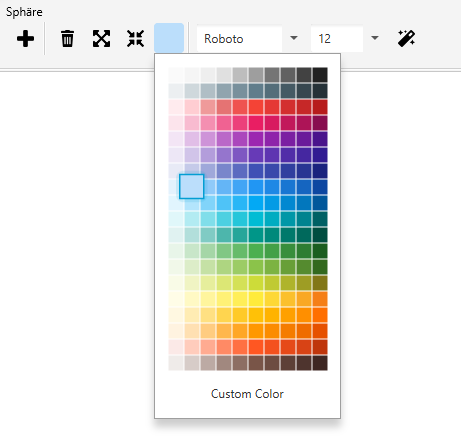
\includegraphics[width=0.4\columnwidth, keepaspectratio]{color.png} 
	}
	\subfigure[Custom Color]{
		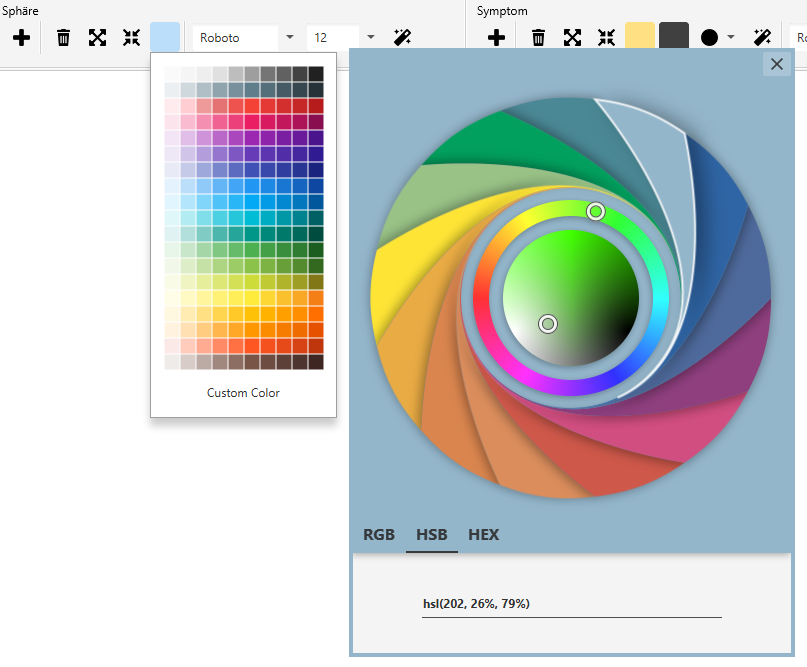
\includegraphics[width=0.4\columnwidth, keepaspectratio]{color2.png} 
	}
	\caption{Color Picker}	
\end{figure}


%%%%%%%%%%%%%%%%%%%%%%%%%%%%%%%%%%%%%%%%%%%%%%%%%%%%%%%%%%%%%%%%%%%%%%%%%%%%%%%%%%%%%%%%%%%%%%%%%%%%%%%%%%%%%		
\section{Fehlermeldungen} \label{fehlermeldungen}

Um die Anwendung von \textbf{GraphIt} so einfach wie möglich zu gestaltet, wird der Benutzer auch auf nicht mögliche/ fehlerhafte Aktionen über eine Fehlermeldung hingewiesen. \\
Eine Fehlermeldung erscheint beispielsweise, wenn eine Sphäre auf einer anderen Sphäre hinzugefügt werden soll. Dies ist aufgrund der Erstellungsregeln eines Syndroms nicht erlaubt. Auch wenn beispielsweise versucht wird ein Symptom hinzuzufügen, obwohl die in den Vorlageregeln maximale Anzahl von Symptomen bereits erreicht ist, erscheint eine Fehlermeldung.

\begin{figure}[ht!]
	\centering
	\subfigure[Fehlermeldung]{
		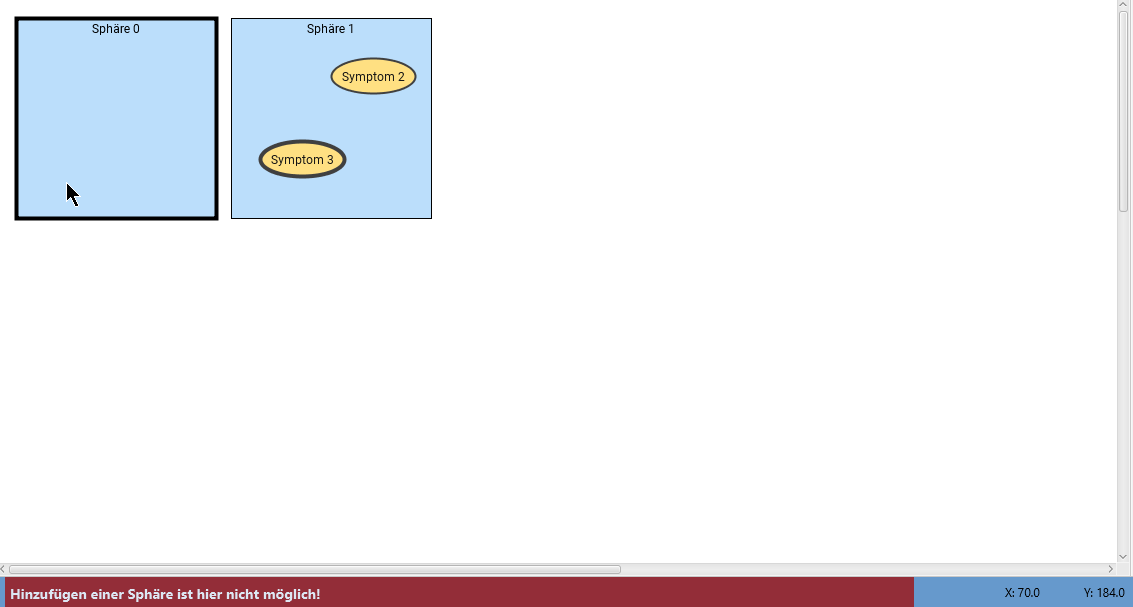
\includegraphics[width=0.9\columnwidth, keepaspectratio]{alert.png} 
	}
	\subfigure[Fehlermeldung(2)]{
		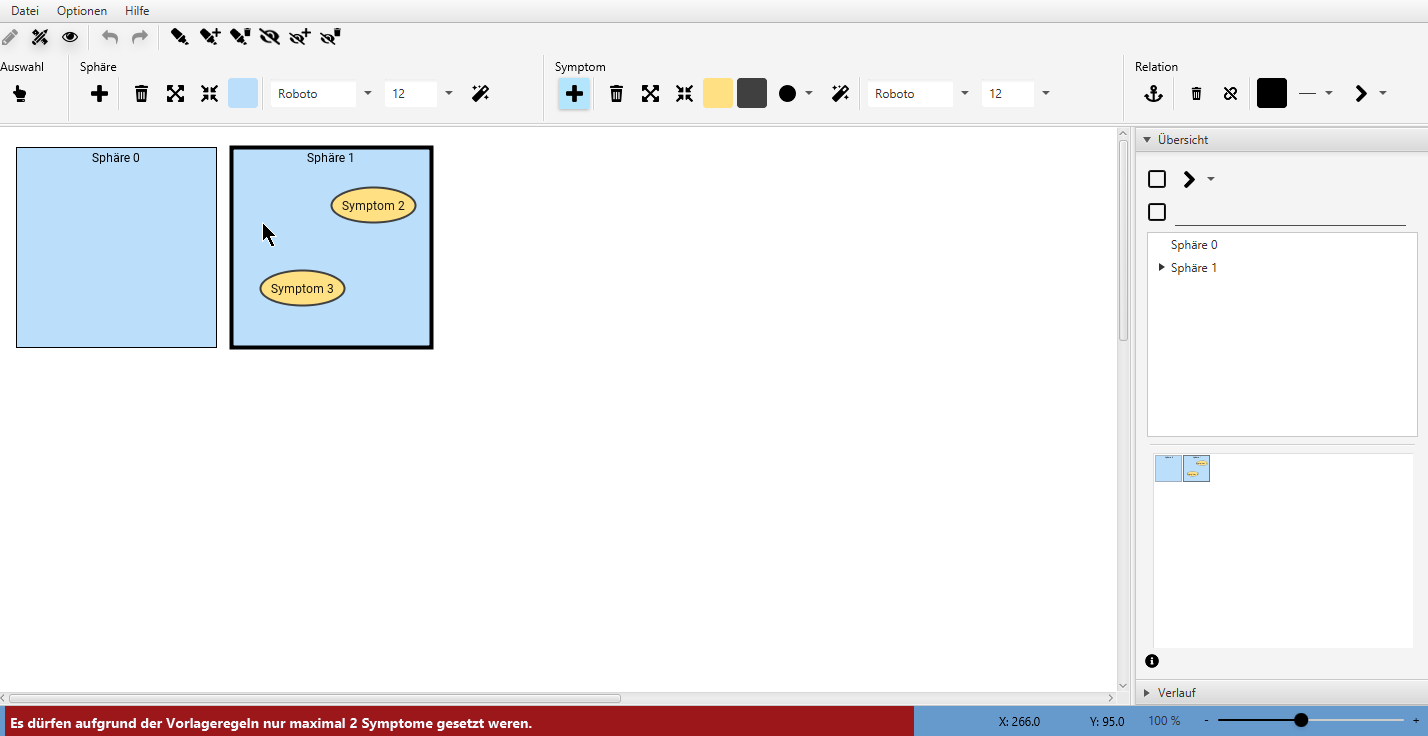
\includegraphics[width=0.9\columnwidth, keepaspectratio]{alert2.png} 
	}
	\caption{Fehlermeldungen}	
\end{figure}

\clearpage
%%%%%%%%%%%%%%%%%%%%%%%%%%%%%%%%%%%%%%%%%%%%%%%%%%%%%%%%%%%%%%%%%%%%%%
\section{Anhang} \label{sec:anhang}	



%%%%%%%%%%%%%%%%%%%%%%%%%%%%%%%%%%%%%%%%%%%%%%%%%%%%%%%%%%%%%%%%%%%%%%%%%%%%%%%%%%%%%%%%%%%%%%%%%%%%%%%%%%%%%		
\subsection{Glossar}
\begin{description}
	\item[Java 8] ist die Version der Programmiersprache Java mit der \textit{GraphIt} programmiert wurde. Java selbst ist eine objektorientierte Programmiersprache. 
	\item[GUI] Graphical User Interface (=Benutzeroberfläche) - hierbei handelt es sich um die Darstellung der für den Nutzer sichtbaren Teile unserer Software. Es dreht sich also bei der GUI um die visuellen Bestandteile des Programms, die es einem Verwender ermöglicht, die Programmfunktionen (intuitiv) nutzen zu können. Vereinfacht ausgedrückt kann in diesem Fall der Nutzer über die GUI einen Graphen erstellen und editieren sowie eine Auswertung des Graph durchführen. 
	\item[GXL] (Graph eXchange Language) ist ein Dateiformat, das dem Austausch von Graphen zwischen Programmen dient. 
	\item[PDF] (Portable Document Format) ist ein plattformunabhängiges Dateiformat, das die Erstellung eines Dokuments ermöglicht, das vom ursprünglichen Anwendungsprogramm losgelöst geöffnet und gelesen werden kann. Das Format gibt dabei den Inhalt des Ursprungsprogramms originalgetreu wieder (sowohl Inhalt als auch Darstellung). 
	\item[.oof] ist ein von uns entwickeltes Dateiformat, das Nutzerinteraktionen und Informationen des Graphen zusammenführt. 
	\item[Graph] ist ein Wirkungsdiagramm und somit eine visuelle Darstellung für den Syndromansatz.  
	\item[\hypertarget{Syndromansatz}{Syndromansatz}] ist ein vom \glqq Wissenschaftlichen Beirat der Bundesregierung Globale Umweltveränderung \grqq{} (WBGU) entwickeltes Modell zur Identifikation von Fehlentwicklungen besonders in den Bereichen Biologie, Gesellschaft und Wirtschaft, um Gegenmaßnahmen planen und durchführen zu können. Es geht hierbei grob gesagt um ein Modell zur Erkennung von \glqq Krankheitsbildern\grqq.
	\item[Syndrom] (=Krankheitsbild) ist ein aus Symptomen (Knoten) und deren Wechselwirkungen (dargestellt über Relationen/Kanten) bestehender Graph in seiner Gesamtheit. 
	\item[\hypertarget{Sphaere}{Sphäre}] ist ein zusammenhängender, nicht-überlappender im Diagramm dargestellter (Themen-)Bereich, zu dem Symptome zugeordnet wird. Sie werden durch Linien voneinander abgetrennt, haben eine wählbare Hintergrundfarbe und können mittels eines Textes beschrieben werden. 
	\item[\hypertarget{Symptom}{Symptom}] ist ein Knoten im Graphen (Syndrom). 
	\item[Relationen] sind gerichtete Kanten von einem Knoten zu einem anderen Knoten im Graphen und dienen der Repräsentation von Wirkungszusammenhängen zwischen Symptomen, wobei zwischen drei Relationstypen unterschieden werden: verstärkend, abschwächend und unbekannt. Die Pfeilspitzen der Relationen sind vom Typ der Relation abhängig und werden ebenso vom Kunden vorgegeben wie mögliche Dicken und Linienarten der Kanten. Die Farben der Kanten können vom Nutzer gewählt werden. Überlappungen von Kantenenden verschiedener Relationstypen, die am selben Knoten eingehen, sind nicht erlaubt.
	\item[Ankerpunkte] sind Stellen an einem Knoten, mit denen der Nutzer den Beginn oder das Ziel einer Kante definieren kann. 
	\item[Pfeilkette] Hiervon ist die Rede, wenn mindestens drei Kanten in dieselbe Richtung zeigen, ohne dass es zu einer Verzweigung bei den inneren Knoten der Kette kommt. Von einem inneren Knoten einer Kette ist ist die Rede, wenn er nicht der Start- und nicht der Endknoten der Kette ist. 
	\item[Verzweigung] Ein Knoten, zu dem zwei oder mehr Kanten hin- bzw. von ihm wegführen, wobei auch beides möglich ist. 
	\item[\hypertarget{Kreislauf}{Kreislauf (Zyklus)}] Eine Kette von Kanten, die geschlossen ist und deren Kanten alle in die gleiche Richtung zeigen. Dabei ist jeder Knoten im Zyklus von jeden anderen Knoten in dem entsprechenden Zyklus aus durch die Kette erreichbar. Eine direkte Rückkopplung ist der kleinste Kreislauf.
	\item[(Nutzer-)Rolle] Wann immer im Dokument von Rollen oder Nutzerrollen die Rede sein wird, ist damit nicht ein Rechtemanagement, sondern vielmehr die Bereitstellung verschiedener Modi gemeint. Jeder Nutzer kann dabei jede Rolle einnehmen und somit das System in jedem Modus verwenden.
	\item[Ersteller- Modus] entspricht der Rolle eines Erstellers. Dieser Modus stellt Funktionen bereit, um ein Diagramm als Vorlage zu erstellen und um bestimmte Bearbeitungsregeln für diese Vorlage festzulegen. Zur Erstellung der Vorlage kann in diesem Modus die Anzahl, Farbgebung und Beschriftung/Benennung der Sphären und Knoten eingestellt und zudem festgelegt werden, welche Kanten verwendet werden können. Optional kann darüber hinaus auch die Größe und Position aller Graph-Elemente sowie der bei der Beschriftung verwendete Zeichensatz ausgewählt werden. Der Verwender dieses Modus kann zudem für jedes Element in der Vorlage einzeln festlegen, ob es einem Verwender im \glqq Diagramm bearbeiten\grqq-Modus gestattet ist, dieses Element zu bearbeiten. Dieser Modus wird üblicherweise von Lehrern zur Erstellung einer Vorlage für ein Diagramm verwendet.
	\item[Bearbeiter- Modus] erfüllt die Ansprüche einer Betrachter-Rolle an das System. In diesem Modus kann ein Benutzer ein Diagramm auf Basis einer Vorlage erstellen und dazu die Vorlage im Rahmen der Regeln aus der gegebenen Vorlage verändern. Ist dieser Modus aktiv, so wird ein Protokoll angelegt, welche Interaktionen des Nutzers in diesem Modus aufzeichnet. Zu den aufgezeichneten Daten gehört ein Zeitstempel sowie die Aktion (z.B. Erstellung, Bearbeitung oder Verschiebung von Sphären, Knoten und Kanten). Dieser Modus ist besonders für Kinder ab 10 Jahren geeignet, die durch ihn komplexe Zusammenhänge verstehen sollen. Um das Verständnis leichter zu machen, sollen auch in diesem Modus bereits \hyperlink{Bedeutung eines Knoten}{gewisse Analyse-Funktionen hinsichtlich der Bedeutung einzelner Knoten} verfügbar sein. Die Analyse-Funktion bezüglich des Protokolls der Nutzerinteraktionen ist nicht verfügbar. Ferner ist alles, was in diesem Modus möglich ist, auch im \hyperlink{``Vorlage bearbeiten''-Modus}{\glqq Vorlage bearbeiten\grqq -Modus} möglich.
	\item[Analyse- Modus] Dieser Modus ist mit einer Auswerter-Rolle vergleichbar. Er stellt Funktionen bereit, um einen erstellten Graphen analysieren zu können (z.B. hinsichtlich der \hyperlink{Bedeutung eines Knoten}{Bedeutung einzelner Knoten}). Diese Analyse beinhaltet darüber hinaus zum einen die Bereitstellung von Möglichkeiten, mit denen man \hyperlink{Metriken}{Metriken/Graphmaße} berechnen kann und zum anderen ein Protokoll, das Aufschluss über die Nutzerinteraktionen (wie zum Beispiel die Reihenfolge, in der Knoten erstellt wurden) gewährt. Dieser Modus wird voraussichtlich von Wissenschaftlern in der Didaktik und eventuell auch von Lehrern verwendet werden.
	\item[\hypertarget{Bedeutung eines Knoten}{Bedeutung eines Knoten}] Die Relevanz eines Knoten ist von der Vernetztheit des Knotens abhängig. Dabei sind mögliche Maßstäbe für Wichtigkeit und Grad der Vernetztheit folgende: Sei K ein Knoten... 
		\begin{itemize}
			\setlength{\itemsep}{0.5pt}
			\item Anzahl der benachbarten Knoten von K (nur Vorgänger, nur Nachfolger, alle Nachbarn)
			\item Anzahl der ein- und/oder ausgehenden Kanten (mit und ohne Abhängigkeit des Relationstyps) von K
			\item Pfeilketten, konvergente und divergente Verzweigungen, Zyklen beliebiger Länge im Graphen
		\end{itemize}
	\item[\hypertarget{Metriken}{Metriken/Graphmaße}] vorgegebene Messgrößen des Syndromansatzes. Man unterscheidet zwischen
		\begin{itemize}
			\setlength{\itemsep}{0.5pt}
			\item \hypertarget{Umfang}{Umfang}: Anzahl wertbarer Symptome + Anzahl wertbarer Relationen (nach Sommer, 2005, S. 151)
			\item \hypertarget{Vernetzungsindex}{Vernetzungsindex}: 2 * Anzahl wertbarer Relationen / Anzahl wertbarer Symptome (nach Ossimitz, 2000, S. 210)
			\item Summer aller Pfeilketten, Verzweigungen und Kreisläufe / Anzahl wertbarer Symptome (nach Kunz \& Bollmann-Zuberbühler, 2008, S. 106)
		\end{itemize}
\end{description}
	

\newpage
\subsection{Referenzen} 
Im folgenden ist die im Dokument erwähnte Fachliteratur gelistet: \\ \\
\begin{tabular}{p{11cm}p{5cm}}
	Werk & wird hier erwähnt \\ \hline \\
	Danny Holten (2006). Hierarchical Edge Bundles: Visualization of Adjacency Relations in Hierarchical Data. In: IEEE Transactions on Visualization and Computer Graphics, 12(5), September 2006, 741-748. ISSN 1077-2626. & \hyperlink{cc}{Überlappung von Knotenenden des selben Relationstyps} \\ \\ 
	Sommer, C. (2005). Untersuchung der Systemkompetenz von Grundschülern im Bereich Biologie.& \hyperlink{Umfang}{Umfang} \\ \\
	Ossimitz, G. (2000). Entwicklung systemischen Denkens. Theoretische Konzepte und empirische Untersuchungen. München: Profil. & \hyperlink{Vernetzungsindex}{Vernetzungsindex} \\ \\
	Kunz, P. \& Bollmann-Zuberbühler, B. (2008): Ist systemisches Denken lehr- und lernbar? In U. Frischknecht-Tobler, U. Nagel \& H. Seybold (Hrsg.), Systemdenken. Wie Kinder und Jugendliche komplexe Systeme verstehen lernen. (S. 33-52). Zürich: Pestalozzianum. & \hyperlink{Strukturindex}{Strukturindex} \\ \\
\end{tabular}


\newpage

\subsection{Abbildungsverzeichnis}
\listoffigures
%%%%%%%%%%%%%%%%%%%%%%%%%%%%%%%%%%%%%%%%%%%%%%%%%%%%%%%%%%%%%%%%%%%%%%
\end{document}


